%%%%%%%%%%%%%%%%%%%%%%%%%%%%%%%%%%%%%%%%%%%%%%%%%%%%%%%%%%
%   Autoren des Abschnitts:
%   Jakob Kautz
%   Olivier Stenzel
%%%%%%%%%%%%%%%%%%%%%%%%%%%%%%%%%%%%%%%%%%%%%%%%%%%%%%%%%%

% !TEX root =  master.tex
\graphicspath{ {./img/} }

\chapter{Konzeption - Hardware}\label{konzeptionHW}~\nocite{*}
\chapterauthor{Jakob Kautz, Olivier Stenzel}
% TODO(Jay): check einheitlichkeit Zeit
% TODO(Jay): Hubmagnet erst nach Unterkapitel Aktuatoren verwenden
% @Note(Val): Abschnitt fängt im Präteritum an und geht dann mit Präsenz weiter
% Glaube, dass Präsenz leichter lesbar ist, aber muss halt einfach einheitlich sei
% @Note(Val): Der ganze Abschnitt argumentiert falsch herum.
% Ihr redet von Aktuatoren, Mikrocontrollern, etc. ohne vorher zu erklären, warum die überhaupt benötigt werden.
% Statt Lösungen zu liefern, sollte hier erstmal erklärt werden, welche Probleme gelöst werden müssen
Für die Umsetzung eines selbstspielenden Klaviers werden verschiedene technische Überlegungen angestellt.
Die Grundfragen, welche bei der Konstruktion auftreten, betreffen die Methode des Anspielens der Klaviertasten, die
Signalübertragung des \ac{MC}s, sowie die Konzeption der Schaltung.
Folgende Anforderungen muss die Konzeption abdecken:
\begin{enumerate}
	\item Ansteuerungskonzept: Die Tasten müssen möglichst effizient von der Hardware angespielt werden, dies beinhaltet Positionierung der Aktuatoren und die Verbindung zwischen Hardware und Klavier.
	\item Auswahl der Aktuatoren: Die Aktuatoren \ref{subsec:aktuator} müssen eine präzise Steuerung der Tasten ermöglichen, ohne dass Akkuratheit und Geschwindigkeit des Anspielens der Tasten vernachlässigt wird
	\item Auswahl des \ac{MC}: Die Aktuatoren benötigen zur Ansteuerung der Klaviertasten die Signale der Software, wobei die Kommunikation via \ac{MC} geschieht.
\end{enumerate}
Die Überlegungen und Entscheidungen für die genutzte Hardware sowie den Aufbau dieser werden in diesem Kapitel erläutert.
Die Hardware-Komponente des Projektes wird im folgenden auch als \enquote{Piano Player} bezeichnet.

\section{Mechanik}\label{konzeptionHW-mechanik}

\subsection{Auswahl des Klaviers}

\chapterauthor{Olivier Stenzel}

Da sich dieses Projekt nicht auf die theoretische Konzeption beschränkt, muss ein entsprechendes Testobjekt - ein reales Klavier - gefunden werden.
Dieses muss einige Voraussetzungen erfüllen:
\begin{enumerate}
	\item 	Der Preis muss im Rahmen des selbst gestellten Budgets (< 2000 €) liegen
	\item 	Es muss leicht auseinander zu bauen sein, damit die Mechanik zugänglich ist
	\item 	Es muss vollständig sein (alle 88 Tasten)
	\item 	Es muss stimmbar sein
	\item 	Der Transport muss einfach durchzuführen sein
\end{enumerate}

Mittels dieser Anforderungen wurde online ein passendes Klavier für 100€ ersteigert.

\subsection{Ansteuerungskonzept} \label{subsec:konzeptionhw-ansteuerungskonzept}

\chapterauthor{Jakob Kautz}

Das Ansteuerungskonzept bezieht sich auf die Problemstellung, dass die Saiten des Klaviers auf irgendeine Art zum
schwingen gebracht werden müssen.
Dafür ist eine Vorrichtung hilfreich, die elektrische Signale in Bewegung umwandeln kann.
Dies ist die Eigenschaft von Aktuatoren, wie z.b. Motoren.

In diesem Kapitel wird untersucht, wie genau man das Anspielen der Saiten technisch umsetzen kann.
Dabei ist eine grundlegende Überlegung, ob man die Saiten direkt anschlägt,
oder die bestehenden Tasten weiter dafür nutzt.

Wenn die Aktuatoren direkt die Saiten des Klaviers anspielen, erfordert dies weniger Kraft im Vergleich zum
Anspielen der Tasten. Das liegt daran, dass die Tasten eine größere mechanische Übersetzung bieten, um die Saiten
anzuschlagen. Wenn die Aktuatoren direkt auf die Saiten wirken, müssen sie nur die erforderliche Kraft aufbringen, um
die Saiten in Schwingung zu versetzen, was im Allgemeinen weniger Kraft erfordert als das Drücken einer Taste mit
ausreichend Kraft, um den Hammer gegen die Saiten zu schlagen.

Die Verwendung von weniger kraftaufwendigen Aktuatoren kann die Gesamtkosten des Systems senken. Aktuatoren, die weniger
Kraft erzeugen müssen, sind oft einfacher und kostengünstiger herzustellen (und zu kaufen) und erfordern möglicherweise weniger
energieintensive Komponenten. Darüber hinaus kann die Verwendung von leistungsschwächeren
Aktuatoren die Größe und das Gewicht des Systems verringern, was zusätzliche Vorteile hinsichtlich Kosten, Transport und
Montage bieten kann. \newline
Allerdings geht dabei die gesamte Mechanik des Klaviers verloren, was bedeutet, dass Aspekte wie Dämpfung nicht genutzt werden können,
was wiederum zu einem weniger ansprechenden Klang führt. Zusätzlich müsste das Klavier permanent geöffnet bleiben, und die
Aktuatoren müssten äußerst präzise die Saiten anschlagen, um akzeptable Ergebnisse zu erzielen.
% @Note(Val): Mit Außnahme des letzten Punkts verstehe ich die Argumente hier ehrlich gesagt nicht. Vieleicht kenne ich mich einfach zu wenig mit Klavieren aus, um das nachvollziehen zu können und wir setzen offensichtlch ein bisschen Klavier-Wissen voraus, aber fals hier für jeden Punkt ein Nebensatz hin könnte, warum das so ist, wäre das wahrscheinlich besser
% @Question(Jay): Ist das so sinnvoller/nachvollziehbarer?
Da der zweite Punkt - ein ansprechender Klang - für dieses Projekt eine höhere Priorität annimmt, fiel die Entscheidung
darauf, die Tasten anzuspielen. Somit kann die Klaviermechanik genutzt werden, was für einen
authentischeren Klang sorgt. \newline
Nun stellt sich also noch die Frage, wie genau die Aktuatoren mit den Tasten des Klaviers verbunden werden.

Eine Möglichkeit besteht darin, die Aktuatoren oben über den Tasten anzubringen, entweder in Form einer nachgebildeten
\enquote{Klavierhand} mit zehn \enquote{Fingern} oder in Form einer Schiene mit 88 Aktuatoren auf den Tasten.
%TODO(Jay): Bilder was ich meine
Beide Lösungen bringen allerdings das Problem mit sich, dass sie gegen die in \ref{sec:zielstellung-anforderungen} definierte Anforderung
der Flexibilität verstoßen, nämlich dass das Klavier sowohl automatisch als auch manuell bespielbar sein soll.\newline
Außerdem würde die Klavierhand-Option - die dem tatsächlichen Klavierspiel ähnlich sieht -
aufgrund der Bewegung und Präzision eine komplexere Logik und
Montage erfordern. Die Schienenoption bietet hier eine viel einfachere Ansteuerung, benötigt jedoch einen Aktuator für jede Taste.
Außerdem steht diese Variante im Gegensatz zu der in Kapitel \ref{sec:zielstellung-anforderungen} Anforderung, dass der Aufbau für unterschiedliche Klaviere anpassbar
sein soll. Das liegt daran, dass diese Schiene eine fest vorgegebene Länge hätte, welche für Klaviere welche eine
andere größe haben, nicht mehr passen würde. \newline

Eine Alternative hierzu besteht darin, die Aktuatoren unter den Tasten anzubringen, wodurch die Anforderung der Flexibilität
im Gegensatz zur ersten Option nicht beeinflusst wird.\newline
Das Klavier kann also sowohl vom \enquote{Piano Player} als auch von einem menschlichen Spieler gleichzeitig bedient werden.
Da diese Anforderung eine hohe Priorität hat, wird die Ansteuerung von untern erfolgen. \newline
Grundsätzlich gibt es hierbei zwei Möglichkeiten für die Ansteuerung:
\begin{enumerate}
	\item Ziehen der Tasten
	\item Drücken der Tasten
\end{enumerate}
Bei beiden Varianten wird jede Taste mit einem Aktuator
ausgestattet, es werden also 88 Aktuatoren benötigt, was die Kosten % @Question(Jay) soll ich späteres Kapitel zu Kosten referenzieren oder so lassen?
im Gegensatz zu der von oben Spielenden \enquote{Klavierhand}
erhöht.
Generell ist die Drückoption ästhetisch ansprechender, da die Hardware sehr einfach versteckt werden könnte.
Somit würde die Illusion entstehen, dass die Tasten sich von alleine bewegen. Die Option erfordert jedoch eine hohe Präzision und könnte die
Tastenempfindlichkeit beeinträchtigen. Außerdem wäre aufgrund der präzisen Montage der Aktuatoren die Anforderung
der Anpassbarkeit (siehe Kapitel \ref{sec:zielstellung-anforderungen}) komplexer umzusetzen.

Für das Drücken der Tasten fallen noch weitere Probleme an. Um die Tasten drücken zu können, muss ein möglichst großer
Hebel aufgebracht werden, damit die Aktuatoren möglichst wenig Kraft für das anspielen aufbrauchen müssen.
Dieser Punkt ist besonders wichtig, wenn der \enquote{Piano Player} mit unterschiedlichen Lautstärken und Dynamiken spielen soll.
% @Question(Jay): Ist es offensichtlich dass das daran liegt dass wir dann auch leiser spielen können oder soll ich das noch erwähnen?
Dies führt dazu, dass die Aktuatoren soweit hinten wie möglich angebracht werden müssen. % @Note(Jay) weil größter Hebel ist offensichtlich, oder?
\newline
% @TODO(Jay): BILD
Hier tritt das Problem auf:
Der Holraum, der sich im hinteren Teil des ausgewählten Klaviers befindet, ist nicht durchgängig. Daher ist es
erforderlich, Löcher einzubauen. Diese müssen räumlich so platziert werden, dass sie keine wichtigen Teile der Klaviermechanik
stören. Aufgrund des Klavierbaus bedeutet dies, dass die Löcher etwa im mittleren Drittel der Taste angebracht werden müssen.
Dies führt zu einer verringerten Hebelkraft. Das Problem betrifft nur etwa ein Viertel der Tasten. Die restlichen könnten mit
voller Hebelkraft von ganz hinten angespielt werden. Allerdings würde dies dazu führen, dass die Tasten
\begin{enumerate}
	\item unterschiedlich stark angespielt werden und der Klang somit seltsam ist,
	\item der Anstoß der Tasten genormt wird und somit nicht die gesamte Dynamik der hinten angebrachten Aktuatoren genutzt
	wird, damit alle gleich klingen. Dies würde die Software komplexer machen, da dies berücksichtigt werden muss, um eine
	konsistente Leistung zu gewährleisten.
\end{enumerate}
Zur Vereinfachung wäre es daher sinnvoller, alle Tasten von der gleichen Höhe aus anzuspielen. Dies bedeutet, dass alle
Tasten von weiter vorne angespielt werden und somit ein Teil der möglichen Dynamik verloren geht. \newline

Diese Probleme fallen beim Ziehen der Tasten weg beziehungsweise sind weniger ausgeprägt. % @Note(Val): Klingt ein bisschen repetetiv mit den vorherigen Sätzen, inhaltlich aber ok
Bei der Präzision liegt der Grund dafür darin, dass die Taste nicht
direkt getroffen werden muss. Stattdessen wird lediglich ein Seil (siehe Kapitel \ref{subsec:VerbindungTastenAktuatoren})
gezogen, das den Aktuator dazu veranlasst, die Taste
gerade nach unten zu ziehen.
Da das Ziehen des Seils weniger präzise Kontrolle erfordert
und keine direkte Interaktion mit der Tastenmechanik erfordert, kann es auch die Tastenempfindlichkeit weniger beeinträchtigen
als das Drücken der Tasten. Es ist allerdings zu beachten, dass das ziehen der Seile - im Gegensatz zum drücken - keine
optimalen Ergebnisse im Bereich des Präzisen spielens bringen. Dies hat mehrere Gründe.
\begin{enumerate}
	\item Verzögerung: Wenn das Seil sich über die Zeit lockert, kann es sein, dass das betätigen der Taste nicht direkt mit der Bewegung des Aktuators kommt. Außerdem würde die Taste so nicht komplett gedrückt werden.
	\item Verschleiß: Die Bewegung über Führsysteme oder Umlenkrollen, welche für eine gerade Bewegung der Seile benötigt werden, können zu Reibungsverlust führen. Außerdem könnten die Seile sich durch verschleiß lockern oder verschieben.
\end{enumerate}
Letztendlich handelt es sich bei beiden Problemen um Gebrauchserscheinungen, welche durch eine gute Auswahl von Seilen
und Wartungen am Klavier wenn es öfter in Benutzung ist minimiert werden können.
Die Hebelkraft ist ebenfalls ein geringeres Problem, da die Aktuatoren Problemlos am vordersten Punkt der Tasten
befästigt werden können, da hier - im Gegensatz zum hinteren Teil des Klaviers - nichts im Weg ist.

Insgesamt fiel die Entscheidung deshalb auf die Strategie des Ziehens von unten.
Bei diesem Ansatz wird die geringste mechanische Präzision benötigt und das Klavier ist trotz Montage des Bots noch manuell spielbar.

\section{Elektronik}\label{sec:konzeptionhw-elektronik}

\subsection{Mikrocontroller}\label{Ansteuerung}
\chapterauthor{Jakob Kautz}
Um die Signale des Programmes an die Aktuatoren weitergeben zu können, ist ein Mikrocontroller (später: \ac{MC}) gut geeignet.
Auf dem Markt steht eine hohe Anzahl an \ac{MC}s zur Verfügung,
wobei für diese Arbeit ein Arduino und ein Rasperry Pi\footnote{Genau genommen handled es sich bei einem Rasperry Pi um einen Einplatinencontroller.} betrachtet wurden.

%Arduino Intro
	\paragraph{Arduino}
	Bei einem Arduino handelt es sich um eine Plattform für die Entwicklung von elektronischen Prototypen. % @Note(Val): Ist ein Arduino wirklich eine "Platform"? Das klingt irgendwie komisch...
	Er besteht aus einem \ac{MC}-Board, das mit verschiedenen Sensoren, Aktuatoren und anderen elektronischen Komponenten verbunden werden kann.
	Der Arduino verfügt über digitale und analoge Ein- und Ausgangspins, die für die Interaktion mit Geräten verwendet werden können.
	\begin{figure}[htbp]
		\centering
		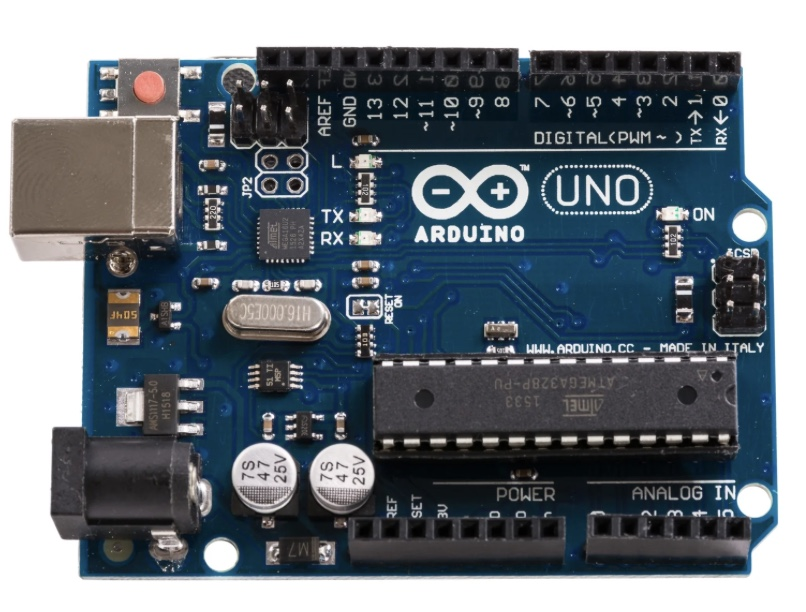
\includegraphics [width=8cm] {img/ArduinoR3}
		\caption{Arduino Uno}
		\label{img:Arduino}
	\end{figure}
\newline
%Pi Intro

\paragraph{Rasperry Pi}
Ein Rasperry Pi ist ein Einplatinencontroller, der auf einem ARM-Prozessor basiert.
Er ist dafür konzipiert, eine breite Palette von Anwendungen zu unterstützen, vom Prototypenbau bis zu IoT-Geräten. % @Question(Val): Sollte IoT ins Abkürzungsverzeichnis?
% @Note(Val): "Im Gegensaz zum Arduino verfügt er über einen Prozessor" - falsch? der Arduino hat offensichtlich auch einen Prozessor...
% @Cleanup(Val): Originaler Satz hier: (angepasst für Abgabe an Kruse für Email)
% Im Gegensatz zum Arduino verfügt er über einen Prozessor und ist besonders für komplexe und rechenlastige Projekte geeignet.
Im Gegensatz zum Arduino ist er besonders für komplexe und rechenlastige Projekte geeignet.
\begin{figure}[htbp]
	\centering
	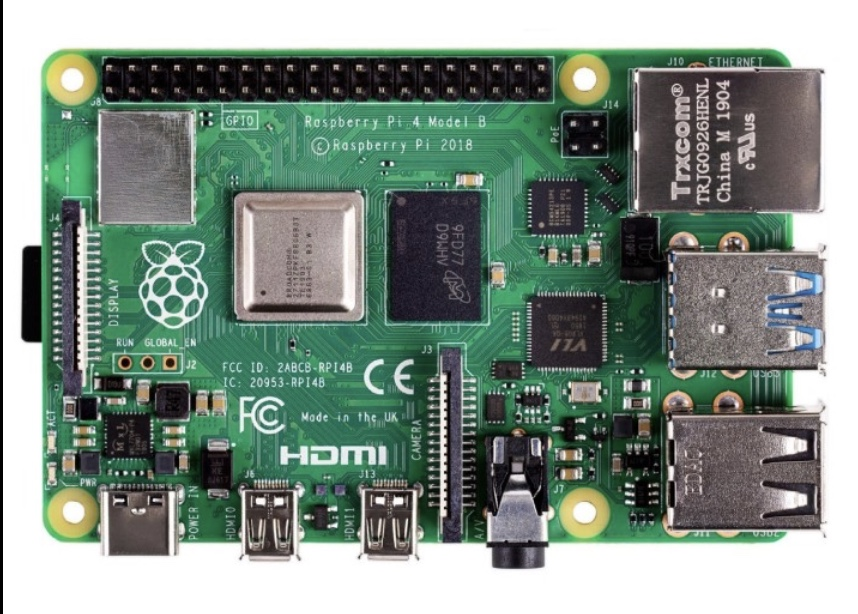
\includegraphics [width=8cm] {img/RasperryPi}
	\caption{Rasperry Pi}
	\label{img:Raspi}
\end{figure}
\newline

%Vergleich
% @Note(Val): Das war der originale Satz, aber der klang sehr komisch...: "Die Entscheidung für den verwendeten \ac{MC} traf auf den Arduino."
Es wurde sich letztendlich für den Arduino entschieden.
Der Rasperry Pi stand vor allem aufgrund seiner höhere Speicherkapazität und Rechenleistung zur Diskussion, wodurch eine komplexere Ansteuerungslogik möglich wäre.
Allerdings ist er aufgrund seines Betriebssystems und einer erhöhten Latenz nicht für Echtzeit-Anwendungen bzw. geschwindigkeitskritische Anwendungen ausgelegt. % @Note(Val): Worauf bezieht sich die Latenz hier genau?
Im Gegensatz dazu bietet der Arduino eine Echtzeitverarbeitung mit geringer Latenz.
Außerdem verfügt ein Arduino über eine recht simple Hardware-Interaktion - er ist darauf spezialisiert, die Hardware direkt anzusprechen - und ist somit besser für Projekte geeignet, welche eine präzise Ansteuerung von Aktuatoren benötigt. % @Note(Val): Simpel != Präzise. Nur weil der Arduino eine simple Hardware-Interaktion hat, heißt es nicht, dass er die Hardware präzise ansteueren könnte
Zudem sollte die Ansteuerungslogik nicht besonders komplex sein, weshalb ein Arduino genug Rechenleistung aufweisen können sollte.

Für das Projekt wird spezifisch ein Arduino R3\footnote{Der Arduino R3 wird auch als \enquote{Mega 2563} bezeichnet.} verwendet.
Bei der Auswahl des spezifischen Arduinos wurden der Arduino Uno, Nano und R3 betrachtet.
Im Prinzip wäre jedes der genannten Modelle für die Anwendung möglich, allerdings verfügt der R3 im Gegensatz zu den anderen beiden Modellen über mehr Speicherkapazitäten (256KB Flash Speicher
gegenüber der 32KB vom Arduino Uno und den 16KB des Arduino Nanos).
Der Arduino Uno verfügt zwar über mehr Ports, allerdings bringt dies keinen Mehrwert, da die Anzahl der benötigten Ausgänge auch bei einem Arduino Uno nicht erreicht werden
(siehe Kapitel \ref{output}).
Der Arduino R3 bietet - wie die anderen beiden Modelle auch - \ac{PWM} Pins, die im Rahmen des Projekts genutzt werden können.
% @TODO(Jay): Add das Arduino CPU-Kern hat

\subsection{Pulsweitenmodulation}\label{PWM}
\chapterauthor{Jakob Kautz}
Zur Vollständigkeit wird in diesem Abschnitt das Prinzip der Pulsweitenmodulation erläutert.
Oftmals ist bei der Ansteuerung der Aktuatoren nicht die gesamte Versorgungsspannung erwünscht bzw. benötigt.
In diesen Fällen muss die anliegende Spannung varriiert werden, damit die Spannung am Ziel dem gewünschten Wert entspricht.
Angenommen es ist eine Spannung von 2.5V erwünscht, wobei die Vollversorgungsspannung 5V beträgt.
Das Signal kann dafür die Hälfte der Zeit ausgeschaltet werden, womit zwischen 0V und den vollen 5V durchschnittlich insgesamt 2.5V anliegen.
Je höher die Frequenz zwischen An- und Ausschalten des Signals eingestellt wird, desto weniger wird diese \enquote{künstlich} simulierte Halbierung wahrgenommen.

\ac{PWM} bedient sich im Grunde genau dieser Technik.
Dabei wird die Zeitdauer eines digitalen Signals variiert wird, um einen durchschnittlichen Wert zu erzeugen.
Bei den \ac{PWM}-Ausgängen wird die Pulsweite - die Dauer der Einschaltzeit - des Signals angepasst, um die gewünschte Spannung zu erreichen.

\begin{figure}[htbp]
	\centering
	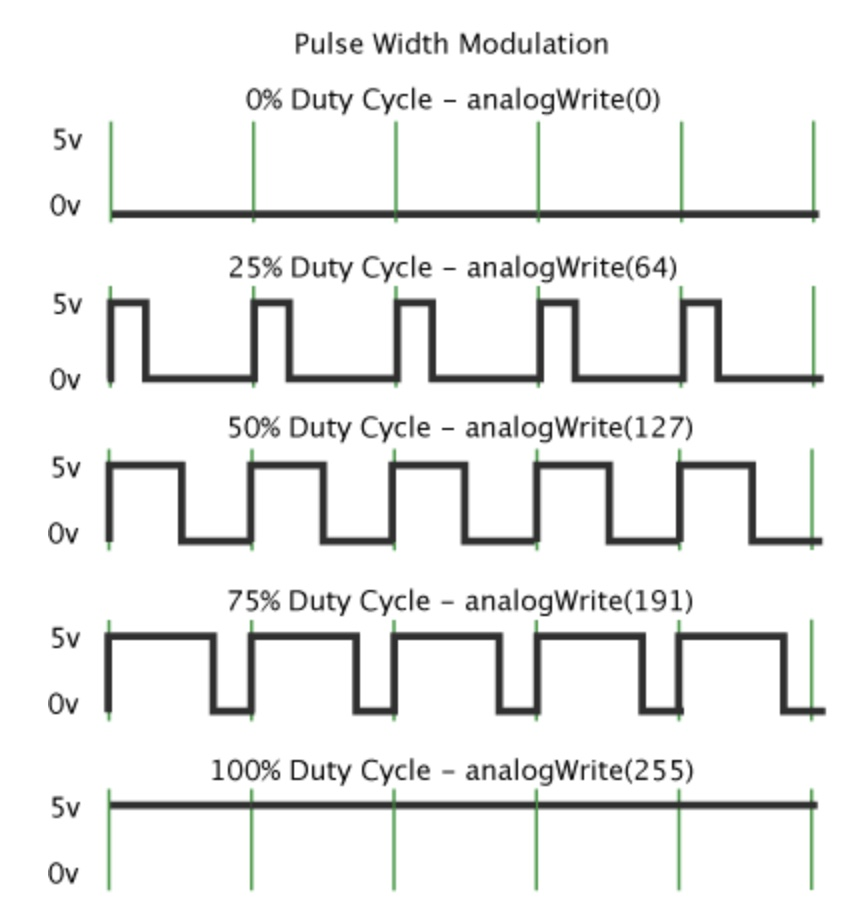
\includegraphics [width=13cm, height=8cm] {img/pulsweite}
	% @Note(Val): Quelle des Bilds fehlt hier noch
	\caption{Pulsweitenmodulation}
	\label{fig:pulsweite}
\end{figure}

Spezifischer ausgedrück passiert folgendes:
Eine digitale Steuerung wird verwendet, um eine Rechteckwelle - ein Signal das zwischen Ein und Aus umgeschaltet wird - zu erzeugen.
Dieses Ein-Aus-Muster kann Spannungen zwischen der vollen Versorgungsspannung und 0V simulieren.
Dabei wird der Anteil der Zeit geändert, für den das Signal eingeschaltet ist relativ zur Zeit, in der das Signal ausgeschaltet ist.
Um unterschiedliche, analoge Werte zu erhalten, wird die Pulsweite moduliert.
Wenn dieses Ein-Aus-Muster zum Beispiel schnell genug mit einer LED wiederholt wird, resultiert daraus eine konstante Spannung zwischen 0 und Vcc, die die Helligkeit der LED steuert.
% @Note(Val): was ist "Vcc" hier? Diese Abkürzung wurde vorher nicht erklärt

% @Note(Val): Hier wechselst du von Ein, Aus zu HIGH, LOW. Einheitliche Benennung wäre hier sinnvoller
Auf den Arduino bezogen sieht die Umsetzung eines \ac{PWM} Signals wie folgt aus:
Ein Taktsignal gelangt in die entsprechende Clock.
Die Clock stellt den entsprechenden \ac{PWM}-Modus ein.
Dabei werden zwei wichtige Werte gesetzt:
Der erste bestimmt, wann das Signal von HIGH auf LOW umschaltet, während der zweite bestimmt, wann es zurückkommt.
Das Verhältnis zwischen HIGH und LOW wird als Tastverhältnis bezeichnet und bestimmt die Helligkeit der LED bzw. die Stärke, mit der der Hubmagnet anschlägt.
Je länger die Ausgabe im HIGH-Zustand bleibt, desto schneller erfolgt der Tastenanschlag.

Neben dem Tastverhältnis, also dem Verhältnis der Einschaltzeit zur Periodendauer, welches oft in Prozent ausgedrückt wird, ist auch die Auflösung ein variierbarer Parameter.
Die Auflösung bezieht sich auf die Anzahl der möglichen diskreten Werte, die das Signal annehmen kann.


\subsection{Vermehrung der Ausgänge}\label{output}
\chapterauthor{Jakob Kautz}
Da ein Klavier über 88 Tasten verfügt, müssen 88 Aktuatoren angesteuert werden. Der gewählte Arduino hat keine 88 \ac{PWM}-Ports, daher
müssen die Signale über eine Erweiterung der Ausgänge an die Motoren weitergegeben werden. Dafür gibt es mehrere Möglichkeiten,
wobei in dieser Arbeit 2 im Detail betrachtet werden:

\begin{enumerate}
	\item Schieberegister
	\item Aktuator-Matrix
\end{enumerate}

% @Note(Jay): Wäre es smart zu erwähnen was es noch für Möglichkeiten gibt? Also Arduino Mega muss ich soweiso erwähnen, aber z.B
% @Note(Jay): Shields verbinden oder mehrere Arduinos nutzen weil das haben wir ja kurz überlegt und dann relativ schnell verworfen

\subsubsection{Schieberegister}
Ein Schieberegister ist ein integrierter Schaltkreis, der zur Speicherung und sequenziellen Verschiebung von
Datenbits verwendet wird.\newline
Das grundlegende Prinzip eines Schieberegisters ist, dass Datenbits seriell in das Register eingegeben und dann
sequenziell aus dem Register ausgegeben werden können.
Dies geschieht durch die Verwendung von Taktimpulsen, die das Verschieben der Bits steuern.\newline
Schieberegister bestehen aus einer Reihe von Flip-Flops.
Ein Flip-Flop kann als ein einfacher Speicher betrachtet werden, der binäre Informationen speichert und je nach
Eingangssignal den Zustand 1, 0, oder einen \enquote{Flip}-Zustand annimmt.
Diese FlipFlops sind so verbunden, dass sie Daten in einer bestimmten Reihenfolge speichern und weitergeben können.

Um 88 Ausgänge mit Hilfe von Schieberegistern, die von nur 3 \ac{PWM}-Pins des Arduinos agesteuert werden, umzusetzen,
können 11 8-Bit-Schieberegister  - also Schieberegister mit 8 Ausgängen - verwendet werden.

\paragraph{74HC959 Schieberegister}
In dieser Arbeit wird spezifisch ein 74HC959 Schieberegister betrachtet.
Dieses hat folgenden Aufbau:
\begin{figure}[htbp]
\begin{minipage}{0.4\textwidth}

		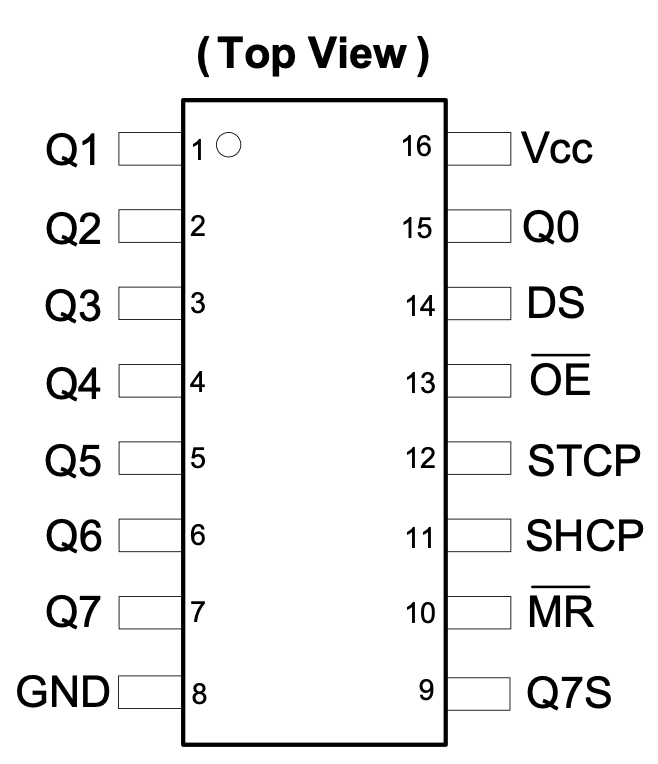
\includegraphics [width=1\textwidth] {img/Schieberegister}
		\caption{Schematik Schieberegister}
		\label{img:Shift}

\end{minipage}
\begin{minipage}{0.6\textwidth}
	\begin{enumerate}
		\item Q0-Q7: Ausgänge (parallelgeschaltet)
		\item Vcc: Anschluss Versorgungsspannung (+)
		\item Gnd: Anschluss Versorgugsspannung (-)
		\item DS: Data Signal, serieller Dateneingang
		\item OE: Output Enable, zur Aktivierung der Ausgänge
		\item SHCP: Shift Clock, Clock-Eingang zur Übernahme Data Signals in Schieberegister
		\item STCP: Store Clock, Beim Wechsel von LOW auf HIgh wird der Inhalt des Schieberegisters in das Ausgaberegister kopiert % @Note(Val): Selbe Bezeichnung wie oben verwenden. Entweder LOW/HIGH oder AN/AUS
		\item MR: Master Reset, Leerung des Schift-Registers
		\item Q7S: Überlauf für Kaskadierung
	\end{enumerate}
\end{minipage}
\end{figure}

% @Note(Val): Kommt hier noch was oder soll das weg?
Vorteile des Schieberegisters:\newline
Nachteile des Schieberegisters:

\subsubsection{Aktuator-Matrix}
% @TODO(Jay): Picture Matrix and use muster to explain it for magnets
Die Aktuator-Matrix ist einer LED-Matrix nachgeahmt.
In einer Matrix, werden zwei Reihen nach folgendem Muster an Ports angeschlossen:
$$
\begin{pmatrix}
	(11) & (12) & (13) & (14) & (15) & (16) & (17) & (18) \\
	(21) & (22) & (23) & (24) & (25) & (26) & (27) & (28) \\
	(31) & (32) & (33) & (34) & (35) & (36) & (37) & (38) \\
	(41) & (42) & (43) & (44) & (45) & (46) & (47) & (48) \\
	(51) & (52) & (53) & (54) & (55) & (56) & (57) & (58) \\
	(61) & (62) & (63) & (64) & (65) & (66) & (67) & (68) \\
	(71) & (72) & (73) & (74) & (75) & (76) & (77) & (78) \\
	(81) & (82) & (83) & (84) & (85) & (86) & (87) & (88)
\end{pmatrix}
$$

Eine LED-Matrix besteht aus einer Anordnung von LEDs in Zeilen und Spalten.
Jede LED kann unabhängig von den anderen ein- oder ausgeschaltet werden.
Die Steuerung der Matrix kann sowohl mit als auch ohne Multiplexing erfolgen.
Prinzipiell wird jede Zeile der Matrix nacheinander aktiviert, während die
entsprechenden LEDs in den Spalten gleichzeitig eingeschaltet werden.
Durch schnelles Wechseln zwischen den Zeilen mithilfe von \ac{PWM}-Signalen erscheint es den Betrachter:nnen, als ob alle LEDs
gleichzeitig leuchten würden, obwohl sie tatsächlich nacheinander aktiviert werden.

\begin{figure}[htbp]
	\centering
	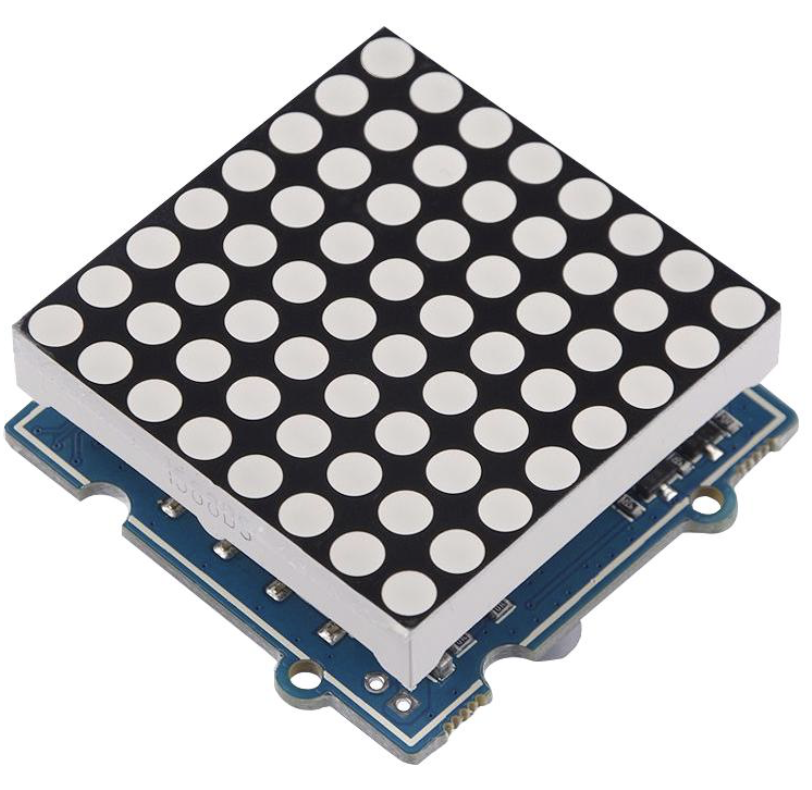
\includegraphics[width=0.45\textwidth]{img/LED-Matrix}
	\caption{Beispielhafte Darstellung einer LED-Matrix}
	\label{img:LED-Matrix}
\end{figure}

%ohne Multiplexer
\paragraph{Matrix ohne Multiplexer}

Bei einer LED-Matrix ohne Multiplexer werden die LEDs direkt über die GPIO-Pins (General Purpose Input/Output) des % @Note(Val): Warum GPIO nicht mit in die Abkürzungen nehmen und dann \ac{GPIO}-Pins schreiben?
\ac{MC}s angesteuert. Jede LED ist einzeln mit einem Pin des \ac{MC}s verbunden. Um die LEDs anzusteuern,
muss der \ac{MC} jeden Pin einzeln aktivieren oder deaktivieren, um die entsprechende LED ein- oder auszuschalten.
Hierbei werden viele Pins benötigt, um die gesamte Matrix anzusteuern, was besonders bei größeren Matrizen unpraktisch
sein kann. Für dieses Projekt, wird wie oben aufgeführt, eine 8x8-Matrix benötigt. Es werden also 16 PWM-Fähige Pins
benötigt. Der hier verwendete \ac{MC} verfügt allerdings nur über ???? von diesen Pins.

\begin{figure}[htbp]
	\centering
	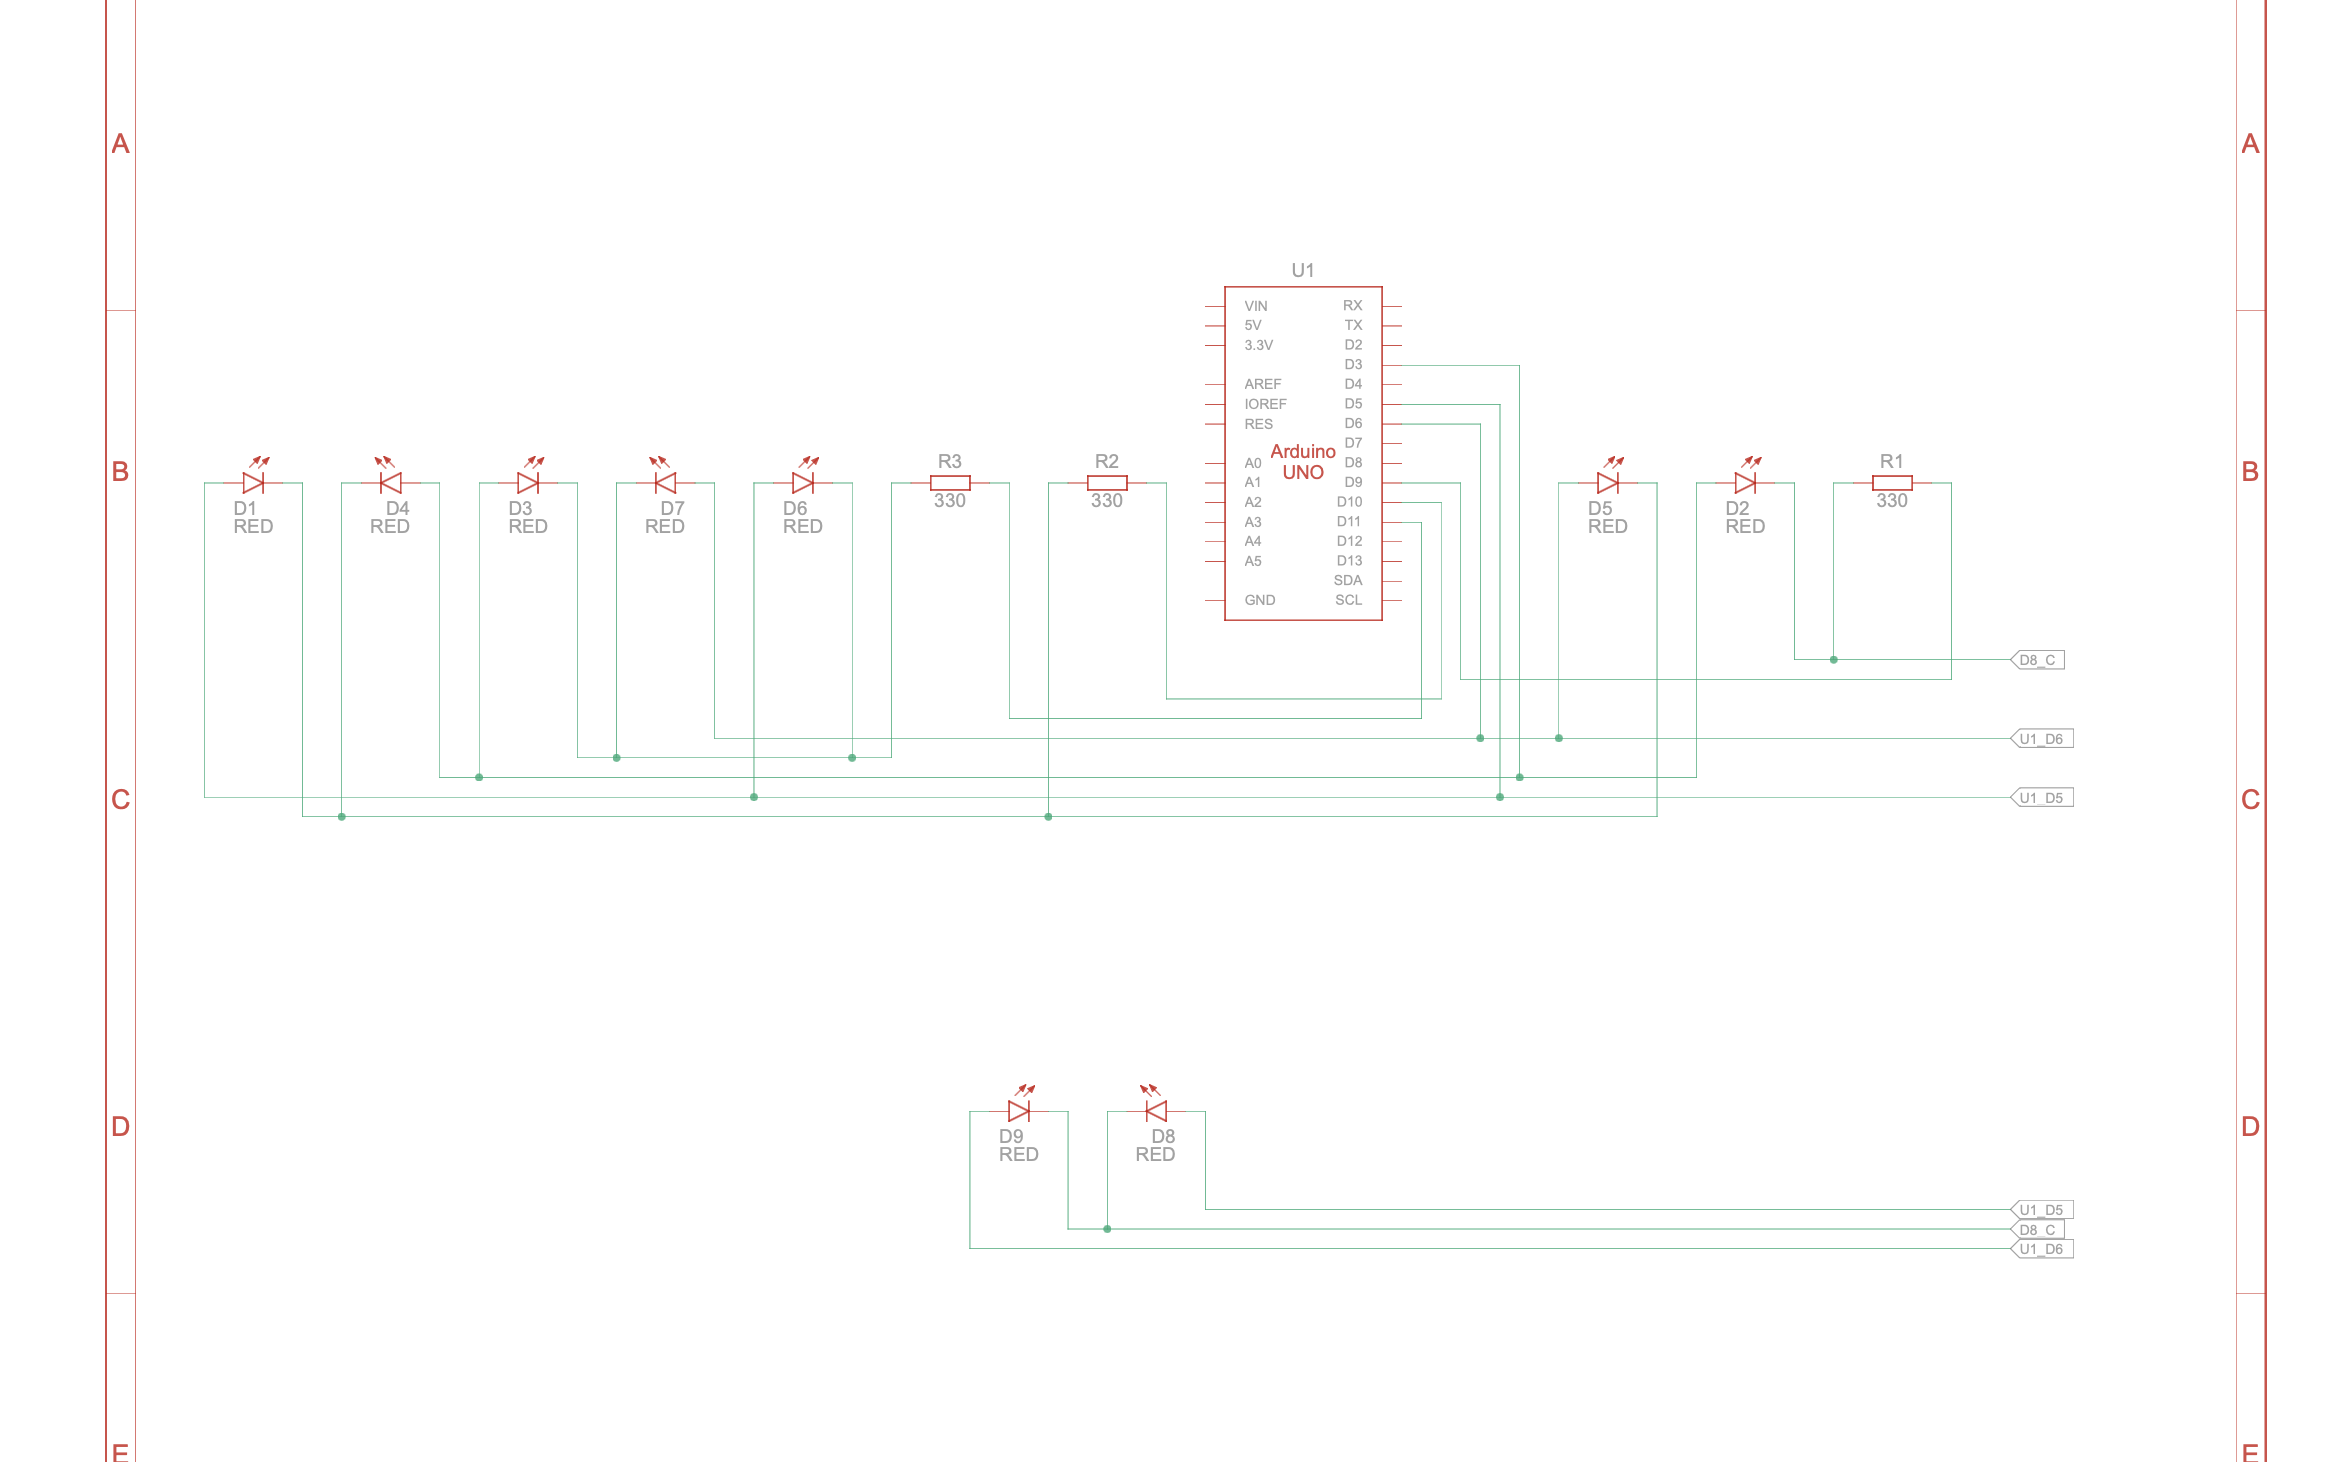
\includegraphics[width=0.75\textwidth]{img/LEDMatrixSchaltung}
	\caption{Matrix ohne Multiplexer Schematisch}
	\label{fig:Matrix}
\end{figure}
\newpage
%mit Multiplexer
%Was ist ein Multiplexer, warum hilft er bei Martix wie sieht allg Schaltung aus?
\paragraph{Matrix mit Multiplexer}

Ein Multiplexer (bzw. ein Demultiplexer) ermöglicht das kombinieren mehrerer Signale zu einem bzw. dem Trennen eines einzelnen Signals zu mehreren, unterschiedlichen Signalen.
Bei einer LED-Matrix kann damit die Notwendigkeit zum Verbinden jedes individuellen Pins mit einem GPIO-Pin des \ac{MC}s elimniert werden.
Entsprechend werden weniger Pins benötigt, um die Matrix anzusteuern.
Die Nutzung von Multiplexern bringt somit eine effizientere Ressourcennutzung mit sich, kommt allerdings auch mit einer komplexeren Schaltung und möglichen Latenzen einher. % @Note(Val): Sind die Latenzen nur "möglich"? Müsste es nicht entweder klar Latenzen erhöhen oder nicht?
\newline
Um die Komplexität darzustellen, eine Aktuator-Matrix ohne Multiplexer würde für neun Aktuatoren wie folgt aussehen:
\begin{figure}[htbp]
	\centering
	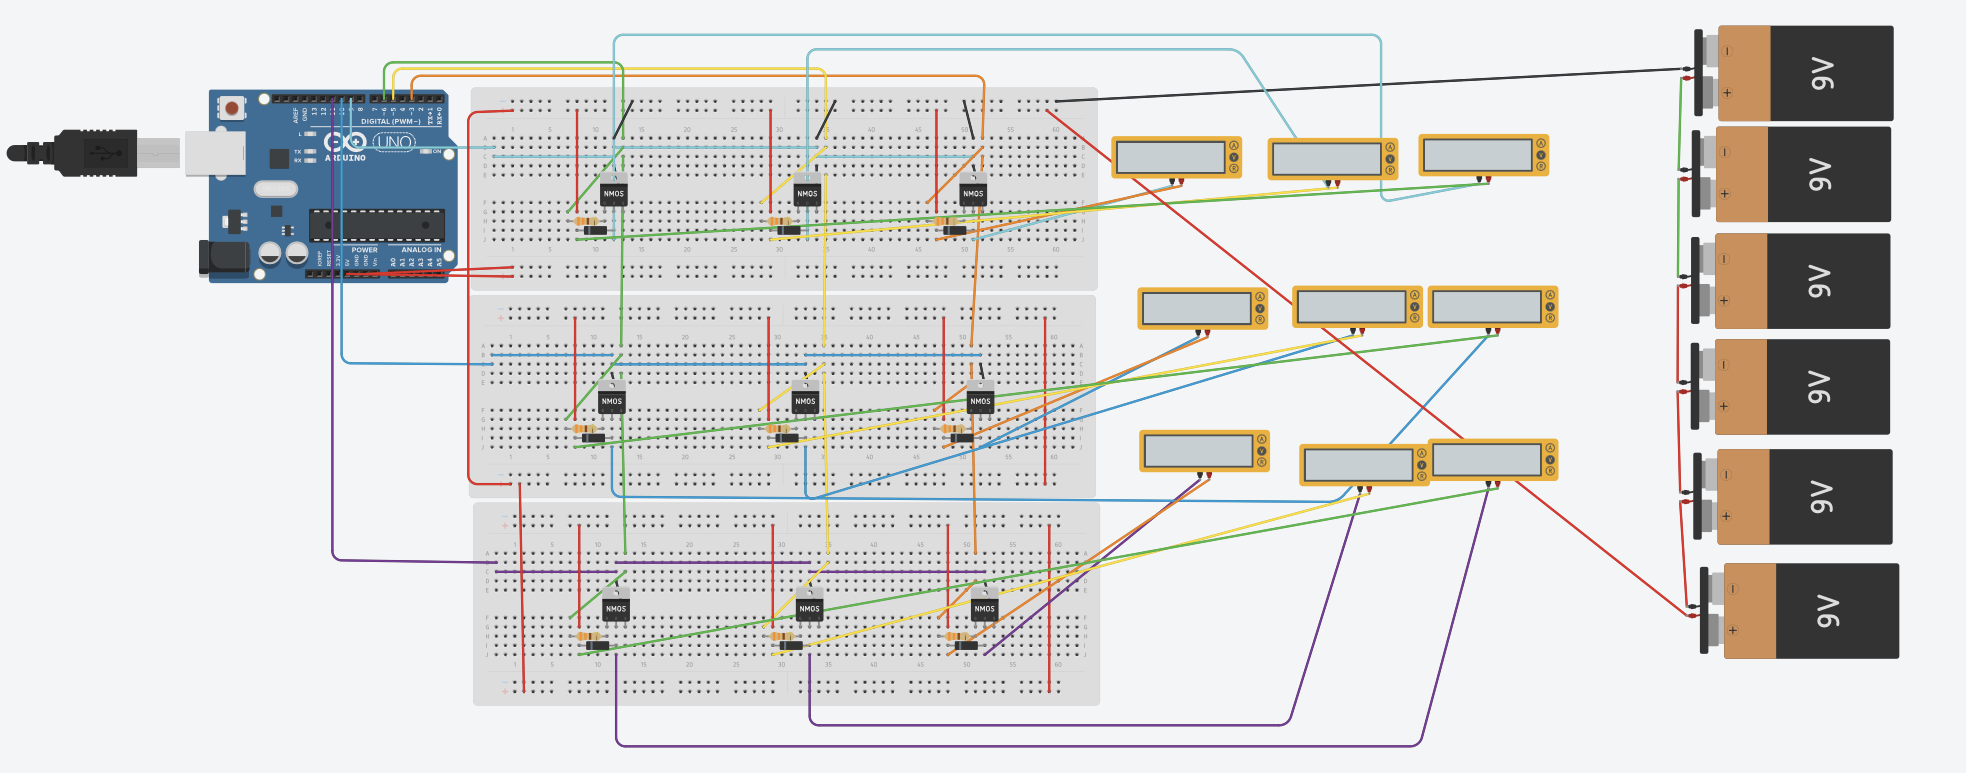
\includegraphics[width=0.9\textwidth]{img/AktMatrix}
	\caption{Aktuator-Matrix ohne Multiplexer}
	\label{fig:AktMatrix}
\end{figure}

\subsubsection{Entscheidungsfindung}

% @Note(Val): Die Aktuatoren wurden bereits entschieden und da es hier teilweise um deren spezifischen Eigenschaften geht (z.B. wie viel Strom sie brauchen) ist es vllt besser von Hubmagneten zu sprechen. Aktuatoren im Allgemeinen benötigen ja nicht unbedingt mehr Strom als LEDs z.B.
Nach weiterer Evaluation der Matrix schien es aus mehreren Gründen schwer möglich, das Prinzip von LEDs auf Aktuatoren
zu übertragen, weswegen die Entscheidung auf die Verwendung von Schieberegistern fiel. \newline
Eine LED-Matrix wird, wie bereits erklärt,
typischerweise durch \ac{PWM} angesteuert, um den Eindruck zu erwecken, dass alle
LEDs gleichzeitig leuchten, obwohl sie tatsächlich nacheinander aktiviert werden. Dieses Prinzip funktioniert gut für LEDs,
da sie einen langsamen Reaktionsmechanismus haben und das menschliche Auge träge ist.
Beim präzisen Ansteuern von Aktuatoren bringt dieses Prinzip jedoch einige Probleme mit sich:

\begin{enumerate}
	\item Stromversorgung und Energieeffizienz: LED-Matrizen werden oft mit einer relativ niedrigen Leistung betrieben. Aktuatoren benötigen dagegen eine höhere Stromversorgung,
	um eine ausreichende Leistung für den Betrieb zu gewährleisten. Die Schaltung, die für eine LED-Matrix optimiert ist,
	könnte möglicherweise nicht die erforderliche Leistung für die Aktuatoren liefern. % @Note(Val): "möglicherweise"? Das klingt als Wissen wir es nicht. Aber wenn wir es nicht wissen, könnte es ja auch besser sein. Und warum wissen wir es nicht? Muss man das unbedingt testen oder was?
	\item Interferenz und ungenaue Steuerung durch die Matrixstruktur: Bei der Verwendung einer Aktuatoren-Matrix über \ac{PWM}
	könnte es zu Interferenzen kommen, die die Präzision der Steuerung beeinträchtigen. Da die \ac{PWM}-Signale zeilenweise
	multiplexiert werden, kann es vorkommen, dass die \ac{PWM}-Signale nicht mit der benötigten Stärke für jeden Aktuator geliefert
	werden. Das liegt daran, dass verschiedene Aktuatoren in derselben Zeile unterschiedliche \ac{PWM}-Signale benötigen können,
	was zu ungenauer Steuerung führen kann. Dies kann zu Kompromissen bei der Präzision und Leistung der Aktuatoren führen. % @Note(Val): Verstehe ich nicht. Jede LED auf der Matrix kann doch unabhängig der anderen angesteuert werden und andere Signale erhalten. Sonst wäre das ja eh nicht nutzbar für uns.
	% @Note(Val): Wieder viele Konjunktive. Entweder es ist ein Problem oder nicht.
	\item Feedback und Regelung: Präzise Aktuatoren erfordern oft ein Feedbacksystem, um ihre Position oder andere Parameter
	zu überwachen und gegebenenfalls anzupassen. Das Zeilenmultiplexing via \ac{PWM} bietet jedoch keinen einfachen Weg, um ein
	solches Feedback zu integrieren, was die Regelung der Aktuatoren erschweren könnte. % @Note(Val): Vorhin wurde doch nur beim Servo-Motor gesagt, dass es ein Feedback-Mechanismus hat. Aber wir verwenden ja Hubmagnete, die vermutlich dann kein Feedback brauchen. Deswegen hier genauer sein als "Aktuator"
	\item Komplexität der Schaltung bei selbstgebauter Aktuator-Matrix: Die Implementierung einer Aktuator-Matrix über eine
	LED-Matrix hinaus wäre technisch anspruchsvoller und erfordert eine komplexere Schaltung. Im Gegensatz dazu ist die
	Verwendung von Schieberegistern eine einfachere (und bewährte) Methode zur Ansteuerung der Aktuatoren. Der Einsatz von % @Note(Val): inwieweit sind Schieberegister hierfür bewährt?
	Schieberegistern vereinfacht die Schaltung und erleichtert die Steuerung der Aktuatoren, was insgesamt zu einer
	zuverlässigeren und Lösung führt. % @Note(Val): Du wiederholst dich 2-3 mal, wenn du sagst dass Schieberegister einfacher sind, erklärst aber nicht warum die Matrix eine komplexere Schaltung benötigt
	\item Anzahl der Pins: Wie bereits erklärt, benötigt die Matrix eine Vielzahl an Pins, welche der \ac{MC} % @Note(Val): Dieser letzte Punkt ist valide aber können wir mMn auch auslassen, wenn wir genug andere Punkte haben
	nicht liefert. Da die Matrix verwendet werden sollte um eben dieses Problem zu lösen, schien es nicht sinnvoll
	das Prinzip einzusetzen. % @Note(Val): Aber mit Multiplexer braucht es doch nicht mehr so viele Pins, oder? Vielleicht konkret berechnen wie viele Pins dann benötigt wären und sagen, dass es immer noch mehr Pins sind als beim Schieberegister?
	\item Ressourcen: Desweiteren basiert die Entscheidung auf unzureichenden Ressourcen für die Matrix. Im Internet gab es
	keine ausreichenden Anleitungen/Ressourcen, die die Implementierung einer LED-Matrix mit Aktuatoren ausreichend
	unterstützen würden. Zusätzlich dazu lieferten die Simulationen via Tinkercad\footnote{Tinkercad: https://www.tinkercad.com} keine befriedigenden Ergebnisse
	für die Aktuator-Matrix.
	Im Gegensatz dazu sind Schieberegister gut dokumentiert und es gibt ausreichende Ressourcen, um ihre
	Verwendung für die Ansteuerung von Aktuatoren zu verstehen und umzusetzen.
\end{enumerate}

Die Kombination dieser Faktoren führte zu der Entscheidung, Schieberegister anstelle einer Matrix für die präzise Steuerung der Aktuatoren zu verwenden. % @Note(Val): Wurde davor schon gesagt. Der Satz kann eig weg, können wir aber auch lassen, falls du es so besser zu lesen findest


% @TODO(Jay): Welchen Hubmagneten verwenden wir genau und wie viel Kraft hat dieser

\subsection{Transistor}
\chapterauthor{Jakob Kautz}
Ein Transistor ist ein elektronisches Bauteil, das in der Lage ist, den Stromfluss zwischen zwei seiner Anschlüsse
(den sogenannten Source und Drain) mithilfe eines dritten Anschlusses (der Gate) zu steuern. Es gibt verschiedene Arten
von Transistoren, wobei grob zwischen Transistor und MOSFET unterschieden wird.
Die grundlegenden Prinzipien ihrer Funktionsweise sind allerdings ähnlich.

\begin{figure}[htbp]
	\centering
	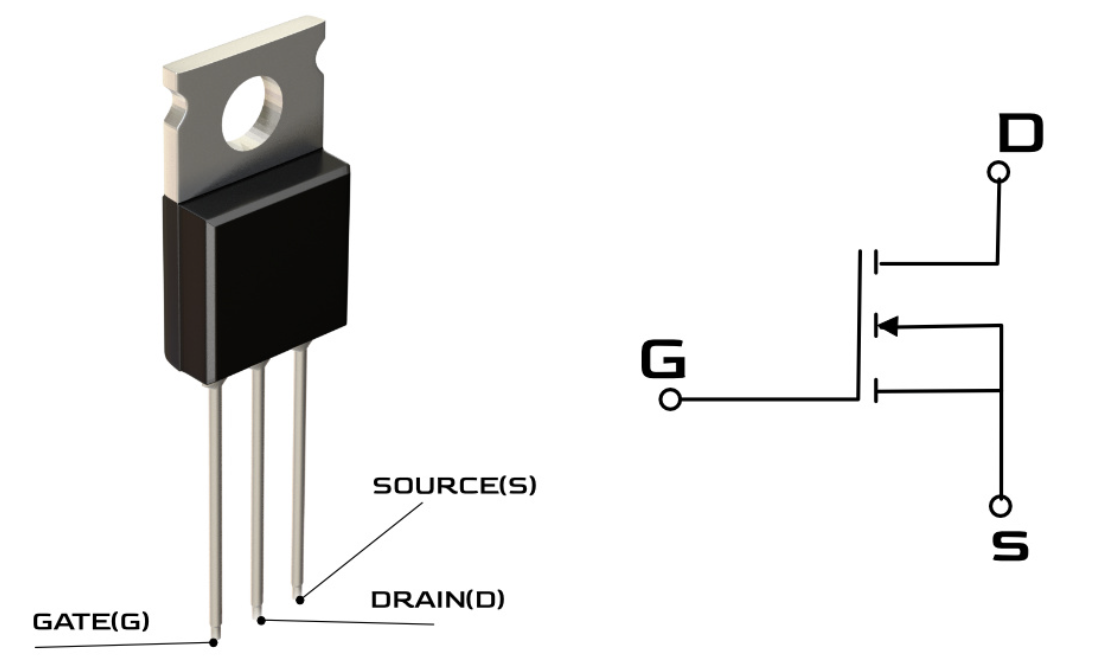
\includegraphics[width=0.45\textwidth]{img/Mosfet}
	\caption{Aufbau MOSFET}
	\label{img:transistor}
\end{figure}

Funktionsweise eines Transistors:
Ein Transistor besteht typischerweise aus einem Halbleitermaterial wie Silizium und kann in drei Haupttypen unterteilt
werden: Bipolartransistor (NPN und PNP) und MOSFET (Metalloxid-Halbleiter-Feldeffekttransistor).  \newline
Bipolartransistor: Die Steuerung des Stromflusses erfolgt durch die Änderung des Stroms, der in die Basis des
Transistors fließt, was den Stromfluss zwischen Emitter und Collector beeinflusst. \newline
%Note(Jay) soll ich Emitter und Collector noch erklären?
MOSFET: Bei einem MOSFET wird der Stromfluss zwischen Source und Drain durch das Anlegen einer Spannung an das Gate
gesteuert, wodurch ein elektrisches Feld im Halbleiter erzeugt wird, das den Stromfluss reguliert. \newline

Unterschied zwischen Transistor und MOSFET: \newline
Ein MOSFET ist eine spezielle Art von Transistor, der auf einem anderen Prinzip basiert als der Bipolartransistor. Der
Hauptunterschied liegt in der Steuerung des Stromflusses: Während beim Bipolartransistor der Strom durch die Basis
gesteuert wird, erfolgt die Steuerung beim MOSFET durch das Anlegen einer Spannung an das Gate.
Bei n-MOSFETs (negativ dotierte MOSFETs, welche in diesem Projekt verwendet wurden) wird durch das Anlegen einer
positiven Spannung am Gate ein
elektrisches Feld erzeugt, das die Leitfähigkeit zwischen Source und Drain beeinflusst. Dies führt dazu, dass der n-MOSFET
in einem bestimmten Bereich des Gate-Spannungsbereichs als Schalter oder Verstärker arbeiten kann. \newline

Verwendung von Transistoren in Aktuatoren-Schaltungen:
Transistoren werden in Aktuatoren-Schaltungen verwendet, um die Aktuatoren
zu steuern. Sie dienen als Schalter, der den Stromfluss zu den Aktuatoren regelt.
Dabei ist es wichtig, auf die Durchlassspannung und Mindestspannung des MOSFETs zu achten. Die Durchlassspannung ist die
minimale Spannung, die an das Gate angelegt werden muss, um den MOSFET in den leitenden Zustand zu versetzen. Die
Mindestspannung ist die minimale Spannung, die zwischen Source und Gate anliegen muss, um den MOSFET zuverlässig zu
sperren.
Es ist entscheidend, sicherzustellen, dass die Spannungen in der Schaltung diese Anforderungen erfüllen, um
eine ordnungsgemäße Funktion des MOSFETs sicherzustellen und Schäden zu vermeiden.

\subsection{Aktuator}\label{subsec:aktuator}
\chapterauthor{Jakob Kautz}
Die Aktuatoren werden für die Steuerung der Tasten benötigt.
Ein Aktuator wandelt Energie in Bewegung (oder andere physikalische Größen) um, um eine gewünschte Aktion herbeizuführen
oder einen Mechanismus zu steuern. \newline % @TODO(Val): Quelle für Aktuator-Definition
Bei den möglichen Aktuatoren für die Ansteuerung der Klaviertasten wurden drei Möglichkeiten betrachtet: % @Note(Val): Falls es einen Grund gibt, nur diese 3 zu betrachten, gerne nennen, ansonsten sollte das auch so fine sein, glaube ich
\begin{enumerate}
	\item Linearmotor % @Note(Jay): Ich glaub es wär smart hier Elektromotor zu sagen und dann zu unterteilen
	\item Servomotor
	\item Hubmagnet
\end{enumerate}

% @TODO(Val): Quelle für jede Definition der 3 Aktuator-Typen
\paragraph{Linearmotor}
Ein Linearmotor ist ein Aktuator, der eine lineare Bewegung erzeugt. Er besteht aus einer festen Spule und einem
beweglichen Magneten oder umgekehrt. Wenn Strom durch
die Spule fließt, erzeugt sie % @Question(Val): Ist es richtig zu sagen, dass die Spule ein Magnetfeld erzeugt? (Ich hab physikalisch keine Ahnung, also kann gut sein, dass das so richtig formuliert ist)
ein Magnetfeld, das den beweglichen Teil des Motors in eine lineare Bewegung zieht. \newline
Physikalische Grundlagen:
\begin{itemize}
	\item Die Funktionsweise eines Linearmotors beruht auf dem Prinzip der elektromagnetischen Induktion. Wenn Strom durch die
	Spule fließt, erzeugt sie ein Magnetfeld, das den beweglichen Magneten anzieht oder abstößt, je nach Polarität des Stroms.
	\item Die Richtung und Geschwindigkeit der Bewegung des Linearmotors hängt von der Stärke und Richtung des angelegten Stroms
	sowie von der Geometrie des Motors ab.
\end{itemize}
\begin{figure}[htbp]
	\centering
	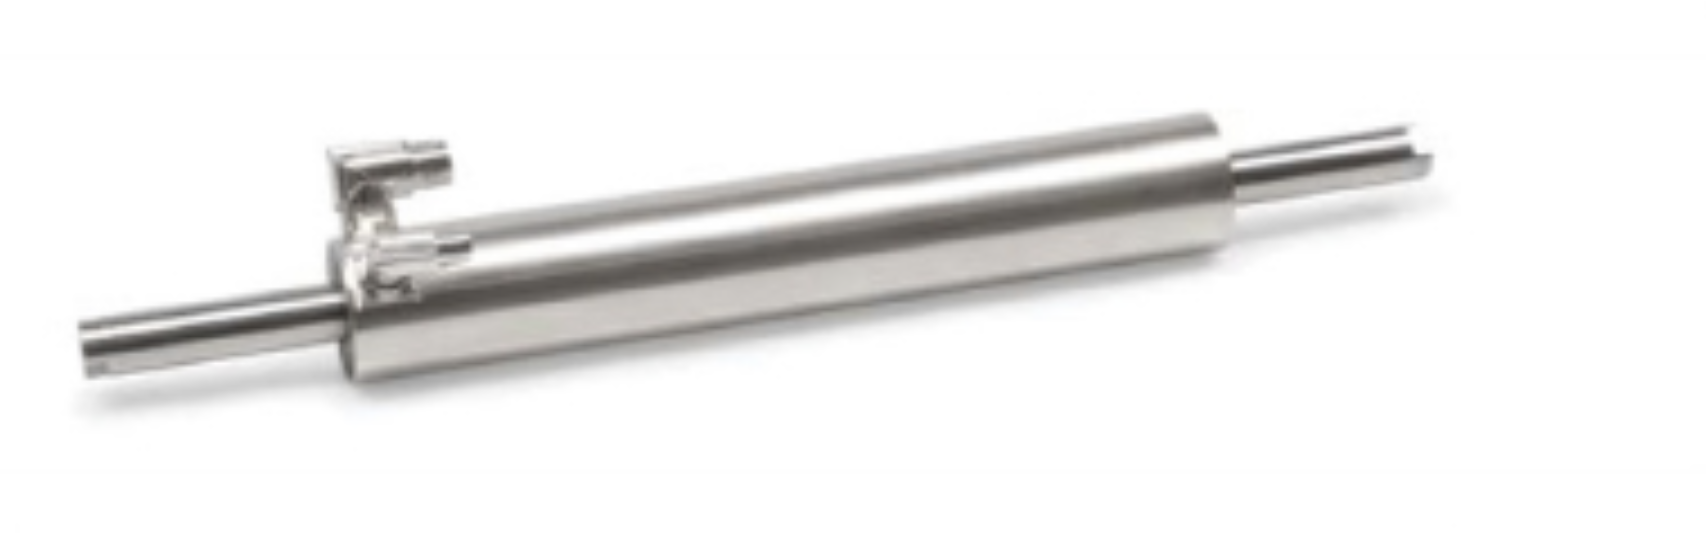
\includegraphics[width=5cm]{img/Linearmotor}
	\caption{Linearmotor}
	\label{fig:Linearmotor}
\end{figure}

\paragraph{Servomotor}
% @Note(Val): Hier scheint etwas falsch zu sein. Bei der Entscheidungsfindung später sagt ihr, dass Servomotoren eine rotierende Bewegung erzeugen. Aber hier sagt ihr, dass es mit einer Drehung anfängt und diese dann vom Servomotor in eine Bewegung (ich nehme an lineare Bewegung) umgewandelt wird.
Ein Servomotor ist ein elektromechanischer Aktuator, der eine Bewegung durch eine Drehung ermöglicht.
Er besteht aus einem Elektromotor, einem Getriebe und einem Feedback-Mechanismus. Der Elektromotor erzeugt eine rotierende
Bewegung, die durch das Getriebe in eine Bewegung umgewandelt wird. Der
Feedback-Mechanismus, oft ein Potentiometer oder ein Encoder, misst die genaue Position des Motors und gibt diese
Informationen an die Steuerung zurück.\newline % @Note(Val): Verstehe nicht inwieweit der Feedback-Mechanismus sinnvoll ist
% @Note(Val): Warum ist das Bild hier zuerst aber ansonsten immer erst nach den physikalischen Grundlgen?
\begin{figure}[htbp]
	\centering
	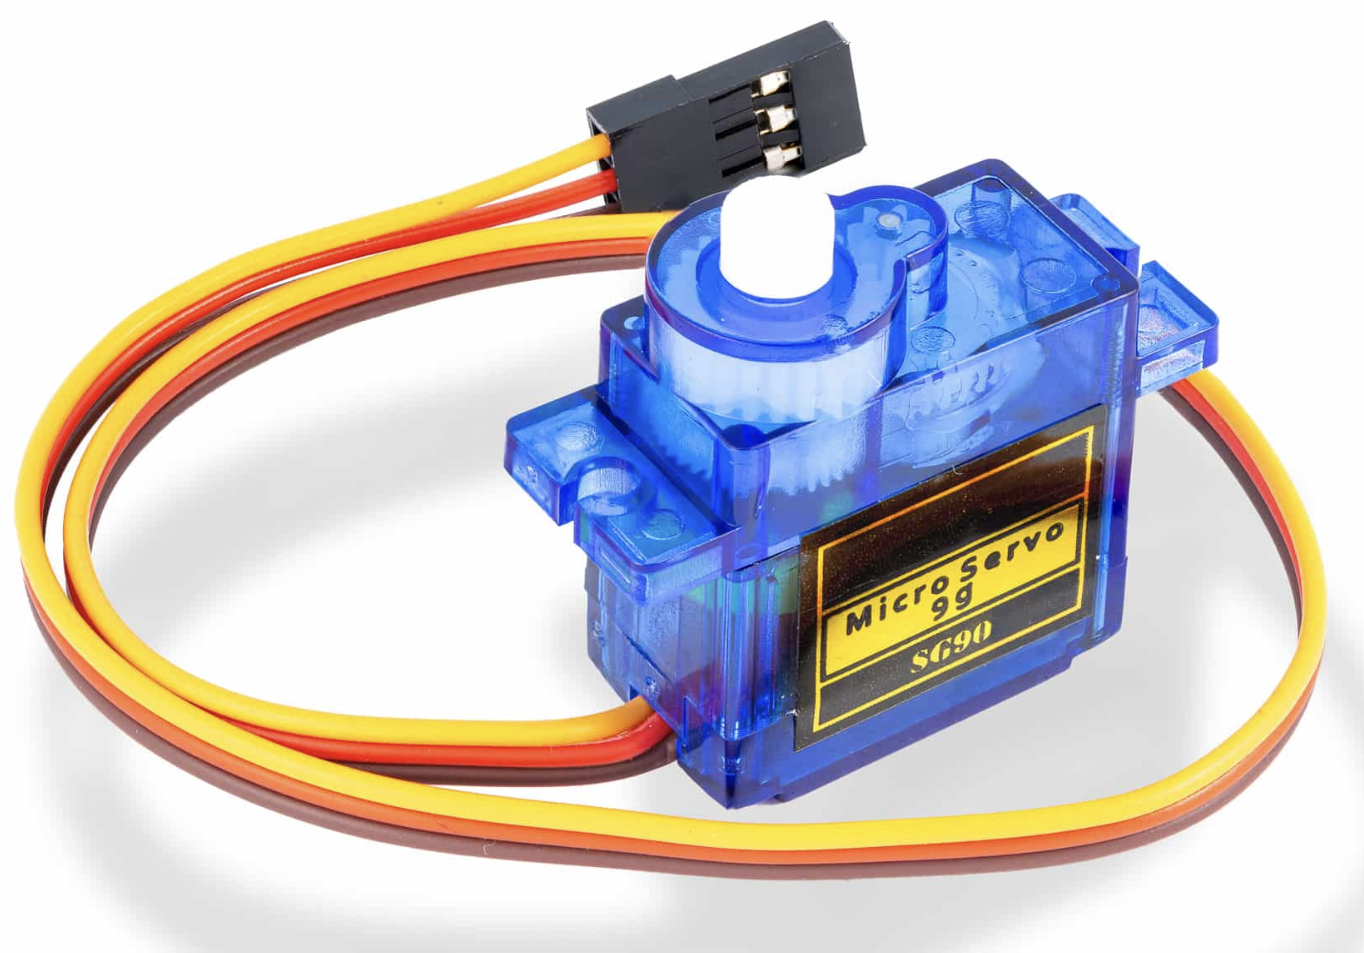
\includegraphics[width=5cm]{img/Servomotor}
	\caption{Servomotor}
	\label{fig:Servomotor}
\end{figure}

Physikalische Grundlagen:
\begin{itemize}
	\item Der Elektromotor nutzt das Prinzip der elektromagnetischen Induktion, um eine Drehbewegung zu erzeugen. Dies geschieht
	durch das Anlegen einer Spannung an die Spulen des Motors, die ein magnetisches Feld erzeugen und den Rotor des Motors in
	Bewegung versetzen.
	\item Das Getriebe dient dazu, die Geschwindigkeit und das Drehmoment des Motors zu regulieren und die Bewegung an die
	Anforderungen der Anwendung anzupassen.
	\item Der Feedback-Mechanismus misst die Position des Motors durch Erfassung von Änderungen des magnetischen Feldes oder der
	Winkelposition des Rotors und ermöglicht so eine präzise Steuerung.
\end{itemize}

\paragraph{Hubmagnet}
Ein Hubmagnet (auch Solenoid genannt) ist ein Aktuator, der eine lineare Bewegung durch das Anlegen eines elektrischen
Stroms erzeugt. Er besteht aus einer Spule, die einen magnetischen Kern umgibt. Wenn Strom durch die Spule fließt, erzeugt
sie ein Magnetfeld, das den Kern anzieht und somit eine lineare Bewegung erzeugt.\newline
Physikalische Grundlagen:
\begin{itemize}
	\item Der Hubmagnet nutzt das Prinzip der elektromagnetischen Induktion, um eine lineare Bewegung zu erzeugen. Wenn Strom
	durch die Spule fließt, erzeugt sie ein Magnetfeld, das den magnetischen Kern anzieht. Je nach Polarität des Stroms bewegt
	sich der Kern entweder in Richtung der Spule oder von ihr weg.
	\item Die Stärke der Bewegung des Hubmagneten hängt von der Stärke des Stroms, der Anzahl der Wicklungen und der
	Spule des Magneten ab.
\end{itemize}
\begin{figure}[htbp]
	\centering
	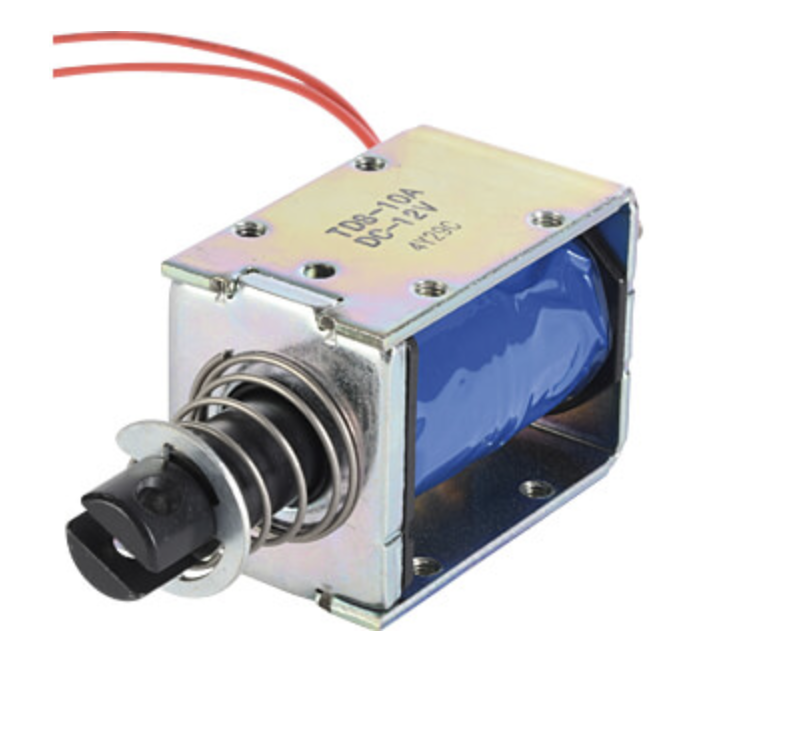
\includegraphics[width=5cm]{img/Hubmagnet}
	\caption{Hubmagnet}
	\label{fig:Hubmagnet}
\end{figure}

Ein großer Vorteil von Hubmagneten ist es, dass beim Anschließen nicht darauf geachtet werden muss, wie rum die
Kabel verbunden werden, weil es
sich um elektromagnetische Komponenten handelt, die auf Basis des elektromagnetischen Prinzips arbeiten. Das bedeutet,
dass der Stromfluss durch den Hubmagneten erzeugt wird, um ein Magnetfeld zu erzeugen, das die Bewegung oder das Halten
von Gegenständen ermöglicht.
Die Polung ist aufgrund der Symmetrie des Magnetfeldes egal:
Das Magnetfeld, das durch den Stromfluss im Hubmagneten erzeugt wird, ist in der Regel
symmetrisch um die Mittelachse des Magneten. Das bedeutet, dass sich die magnetische Kraft gleichmäßig um den Magneten herum
verteilt, unabhängig davon, welche Polung verwendet wird. Daher spielt es keine Rolle, welcher Anschluss an Plus oder Minus
angeschlossen wird, da das resultierende Magnetfeld ähnlich sein wird.

%TODO(Jay): QUELLE

\paragraph{Entscheidungsfindung}
Prinzipiell kann jeder der genannten Aktuatoren für das Projekt verwendet werden. Die Entscheidung fiel aufgrund
mehrerer Vortzeile allerdings auf den Hubmagneten:
\begin{enumerate}
	\item Servo-Motor: Bei diesem Motor ist eine Bewegungsbeschränkung mit eingebaut, welche in jedem Motor ausgebaut
	werden müsste. Dies ist zu umständlich, wenn es bessere Varianten - wie den Hubmagneten - gibt. Außerdem hätte
	eine Umlenkung stattfinden müssen, da die erzeugte Bewegung eine Rotation im Gegensatz zu einer linearen Bewegung
	ist. Zwar gibt es auch lineare Servomotoren, welche allerdings ebenfalls aufgrund ihrer Bewegungsbeschränkung nicht
	weiter betrachtet wurden. % @Note(Val): Warum erwähnt ihr die rotierende Bewegung dann überhaupt als Nachteil. Und warum werden vorher bei der Erklärung nicht die linearen Servomotoren erklärt?
	Zusätzlich verweilen Servomotoren nach ihrer Ansteuerung an der Position, an der
	sie bei Ende der Stromversorgung waren. Für das Klavier werden Aktuatoren benötigt, welche wieder auf die vorherige
	Position zurückschalten, die Klaviertaste also in dem Sinne wieder \enquote{loslassen} können.
	\item Linear-Motor: Auch hier kam das Problem auf, dass die Motoren nicht automatisch wieder an ihre vorherige
	Position zurückschalten, wenn der Stromfluss stoppt. % @Question(Val): Das Problem könnte mit einem gegenteiligen Stromfluss gelöst werden, oder? Weiß aber nicht ob das die Schaltung unbedingt verkomplizieren würde. Wenn das überhaupt nicht möglich wäre, wären Servo- & Linear-Motoren ja gar nicht nutzbar und dann wäre die Einleitung für diesen Abschnitt falsch
	\item Hubmagnete: Hubmagnete sind schneller als die anderen beiden Aktuatoren, was insbesondere bei schnellem
	Tastendrücken sinnvoll ist. Außerdem schalten Sie, wenn die Stromversorgung abbricht, wieder auf ihre vorherige
	Position zurück. Der Nachteil ist, dass Sie allgemein weniger Kraft aufbringen als Servo- und Linearmotoren.
	Da das Anziehen der Tasten allerdings nicht genug Kraft braucht um über diese Schwelle hinauszugehen, führte dies lediglich dazu, dass Kostenintensivere Solenoids bestellt werden müssen.
			% @Note(Val): Der letzte Satz hier ist komisch & wahrscheinlich falsch (was genau bedeutet "genug" hier z.B.)
			% @Note(Val): Der Nachteil ist doch gar nicht, dass sie weniger Kraft aufbringen, wenn es auch Solenoids gibt, die diese Kraft aufbringen, oder? Der Nachteil ist eher, dass die Solenoids, die solche Kraft aufbringen, mehr kosten, oder?
\end{enumerate}


\subsection{Schaltplan} \label{subsec:schaltplan}
\chapterauthor{Olivier Stenzel, Jakob Kautz}

Der Schaltplan besteht im Großteil aus den bereits aufgeführten Komponenten:
\begin{enumerate}
	\item Arduino
	\item Schieberegister
	\item MOSFET
	\item Hubmagnet
\end{enumerate}
In diesem Kapitel wird erläutert, wie diese Komponenten miteinander verbunden werden um eine Funktionsfähige
Schaltung zu erstellen. Die gesamte Schaltung mit allen 88 Hubmagneten wird wie folgt aussehen:
\begin{figure}[htbp]
	\centering
	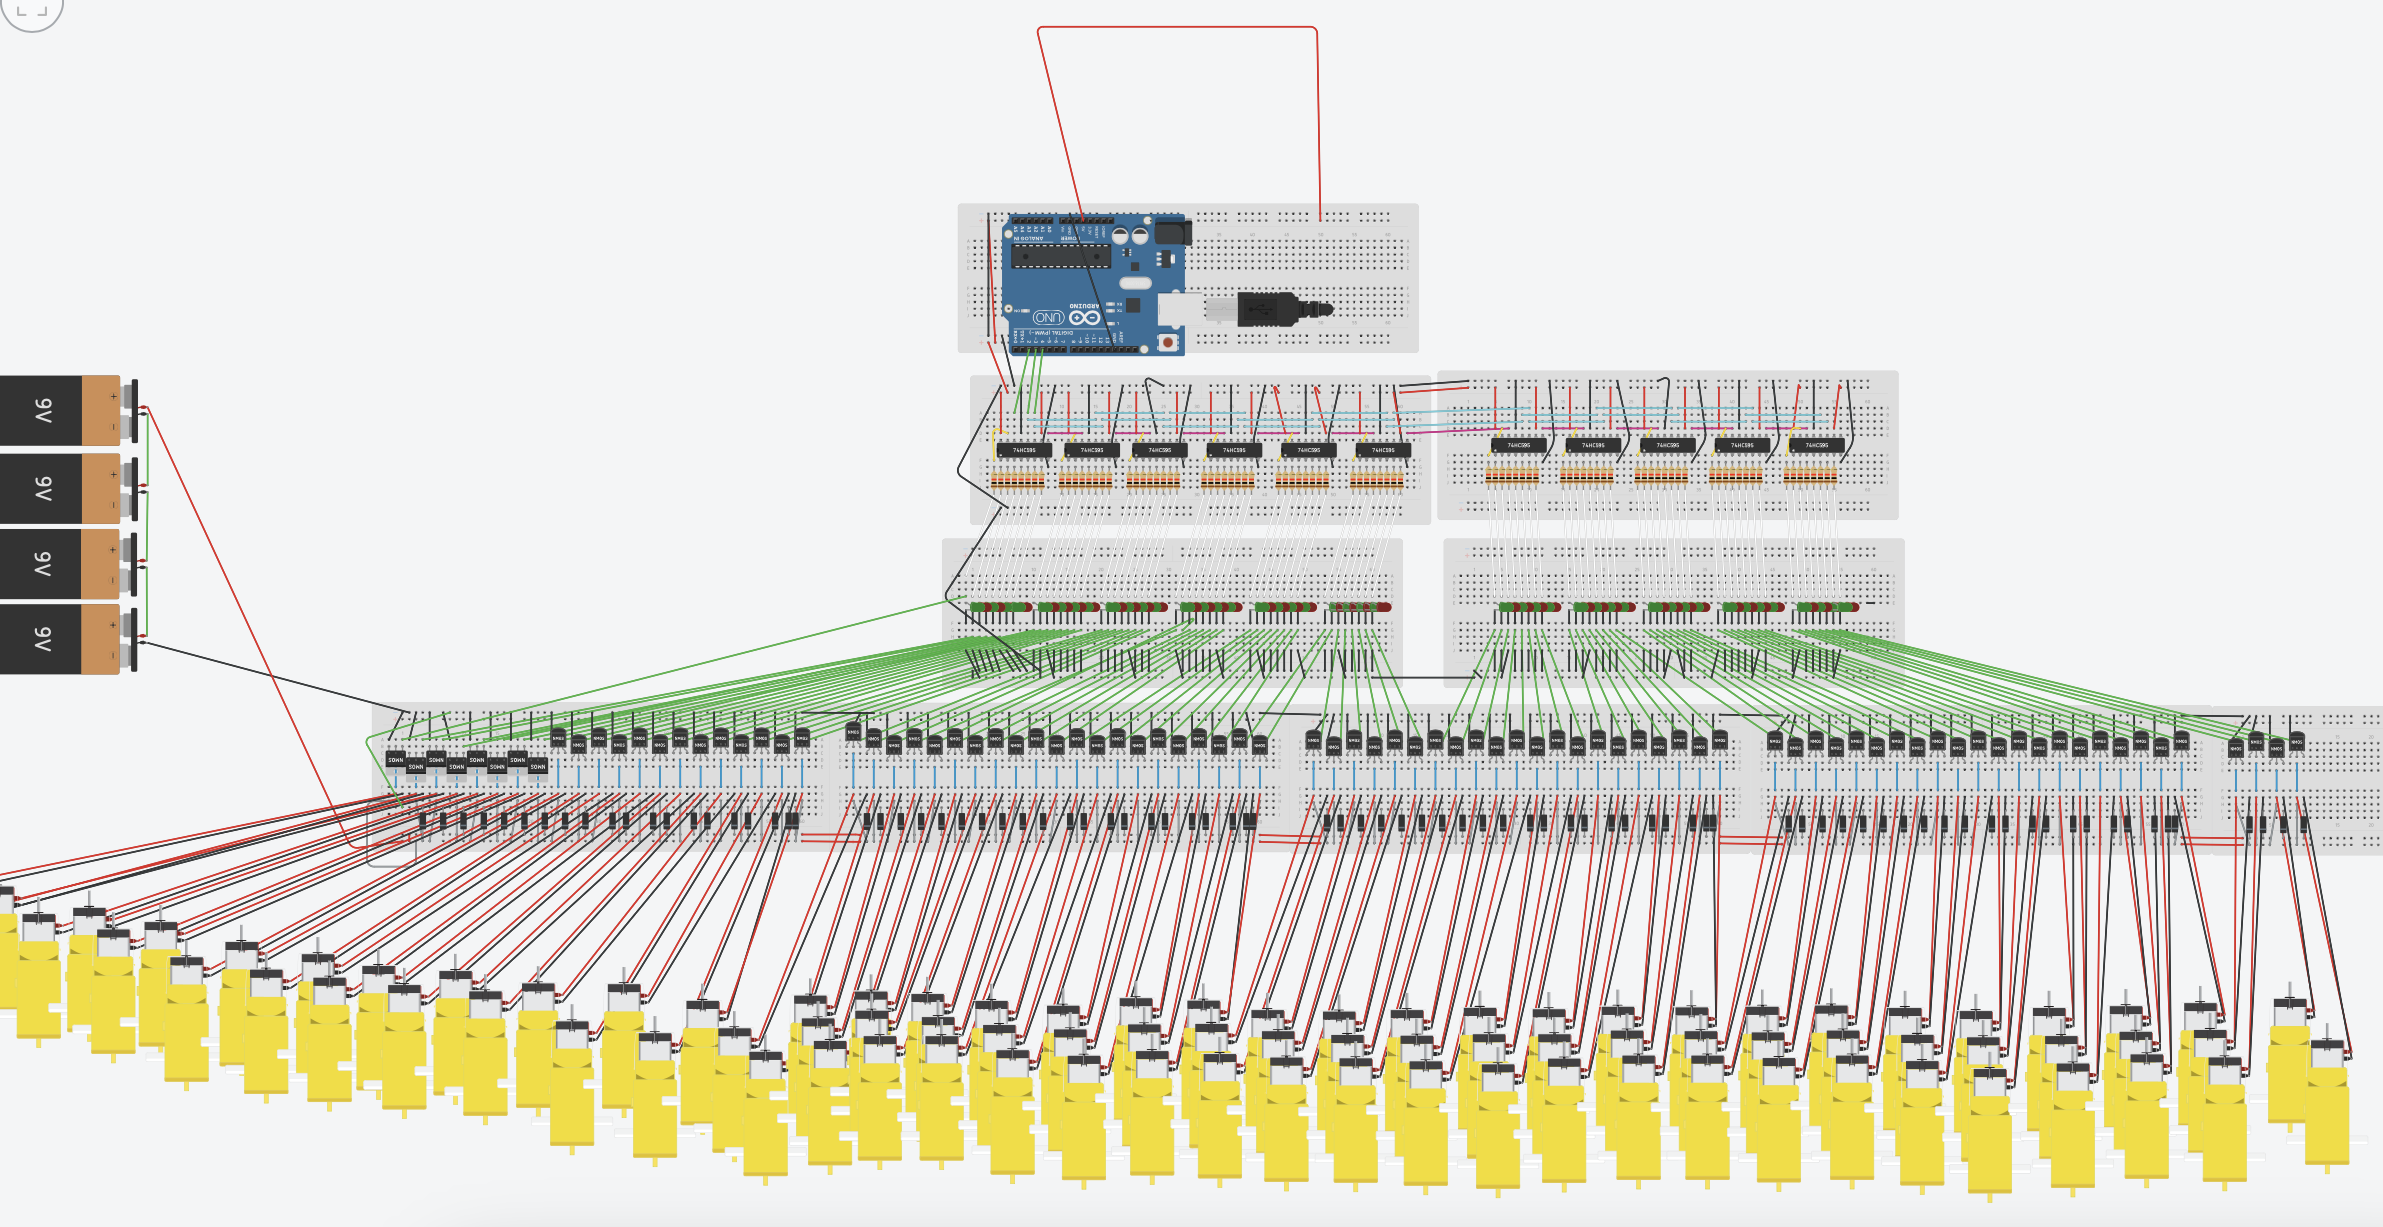
\includegraphics [width=0.85\textwidth] {img/SchaltungGesamt}
	\caption{Überblick Schaltplan}
	\label{img:Schaltplan}
\end{figure}
\subsubsection{Arduino}

Im Zentrum der Schaltung steht der \ac{MC} (hier: Arduino Uno R3).
Dieser erhält Daten und Strom über den integrierten USB-Anschluss, welcher mit dem Computer verbunden wird.
Da der Arduino limitierte \nameref{PWM}-fähige Ausgänge bereitstellt, werde Schieberegister (74HC595) verwendet.
Mit jedem \enquote{in Reihe} geschaltetem Schieberegister kann die Anzahl \ac{PWM}-fähiger Ausgänge um 8 erweitert werden.

\subsubsection{Schieberegister}

Der Arduino wird an fünf Stellen mit dem ersten Schieberegister verbunden:

Arduinoport D2 <-> Serial (SER) Input

Über diese Verbindung werden serielle Daten werden hier bitweise in das Register geschoben.

Arduinoport D3 <-> SHCP (Shift Register Clock Input)

Dieser Pin wird verwendet, um den Takt für das Verschieben der Daten innerhalb des Schieberegisters anzulegen.
Bei jedem Taktimpuls auf diesem Pin wird das Bit am seriellen Dateneingang in das Register verschoben.
Das bedeutet, dass bei jeder steigenden Flanke des Taktsignals das Datenbit, das am Eingang anliegt, in das Schieberegister übernommen und alle vorhandenen Daten um eine Position verschoben werden.

Arduinoport D4 <-> STCP (Storage Register Clock Input)

Nachdem die Daten in das Schieberegister eingelesen wurden, wird dieser Pin verwendet, um die im Schieberegister vorhandenen Daten in das Ausgangsregister zu übertragen.
Ein Taktimpuls auf diesem Pin bewirkt, dass die Daten vom Schieberegister ins Ausgangsregister übernommen werden, sodass alle Ausgänge gleichzeitig aktualisiert werden.
Das ist besonders relevant, da sonst unter Umständen alle Ausgänge von einer Änderung im letzten Schieberegister betroffen wären.

Arduino GND <-> Ground, Output Enable (OE)

Der OE-Pin wird genutzt, um die Ausgänge des Schieberegisters global zu aktivieren oder zu deaktivieren, ohne die Daten selbst zu beeinflussen.
Da das Schieberegister zu keiner Zeit deaktiviert sein soll, wird dieser Pin dauerhaft mit dem GND-Pin verbunden.

Arduino VCC 5V <-> VCC, $\overline{SRCLR}$ (Reset)

Um das Schiebregister mit den benötigten 5V zu betreiben, wird der entsprechende Pin mit dem 5V Output des Arduino verbunden.
Zusätzlich wird der $\overline{ }$ SRCLR Port des Schieberegisters, welcher ein Reset ermöglicht dauerhaft mit 5V verbunden.

Jedes weiteres Schieberegister greift die oben genannten Signale ab.
Der einzige Unterschied befindet sich am Serial (SER) Input Port.
Das Schieberegister an Position i+1 wird mit dem seriellen Output des Schieberegisters an Position i verbunden. ($\forall i = 0,...,10$)

\begin{figure}[htbp]
	\centering
	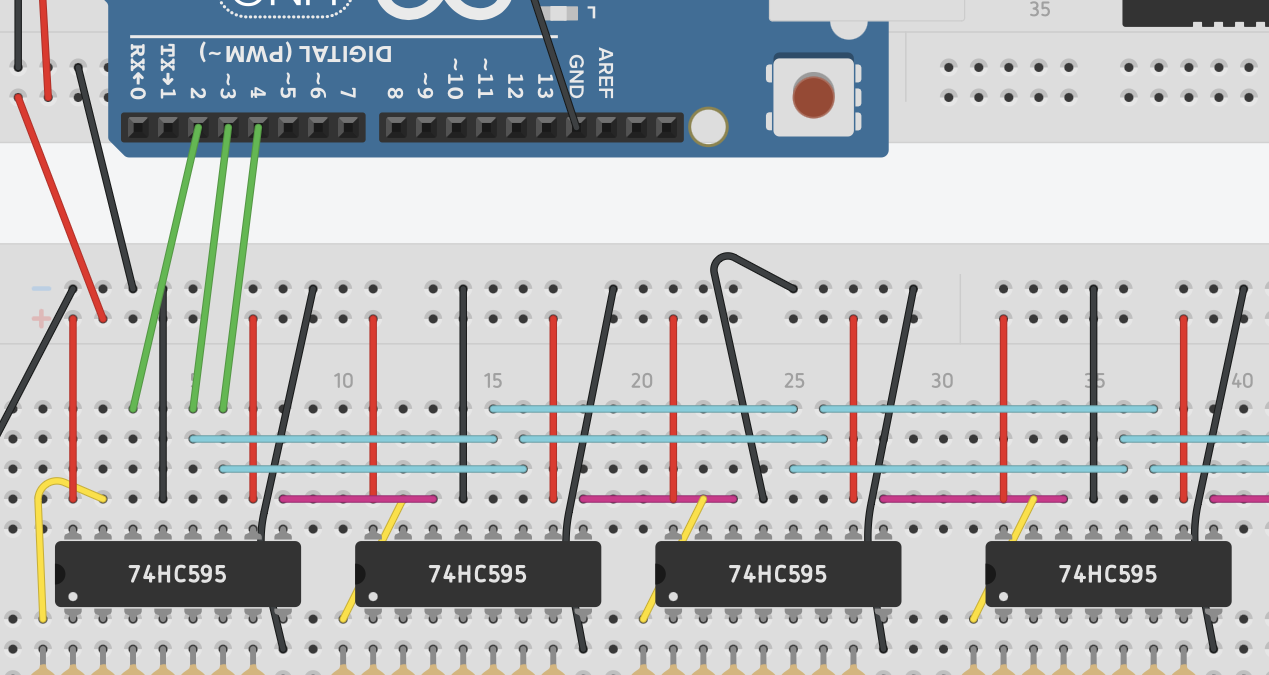
\includegraphics[width=0.9\textwidth]{img/SchaltungSchieberegister}
	\caption{Schaltung der Schieberegister}
	\label{fig:Shifting}
\end{figure}

\subsubsection{MOSFET}

Die Hubmagnete werden jeweils mit 24V und mit bis zu 400mA betrieben.
Um einen hohen Stromfluss zu steuern, können Transistoren verwendet werden.
Für hohe Spannungen und schnelle Schaltvorgänge eigenen sich besonders MOSFETs (Metall-Oxid-Halbleiter-Feldeffekttransistor).
Im Folgenden werden speziell n-MOSFETs verwendet, der mit einem Signal zwischen 0V (leitet nicht) und +5V (voll leitend) angesteuert werden kann.

Der folgende Aufbau ist für die insgesamt 88 Ausgänge der 11 Schieberegister identisch, da jeder Ausgang für die Ansteuerung genau eines Motors zuständig ist.

Der GATE-Pin des MOSFETs erhält das Signal, dass die \enquote{``Durchlässigkeit''} steuert aus einem der Outputs des Schieberegisters.
Der SOURCE-Pin wird mit Ground des gesamten Systems verbunden.
Der DRAIN-Pin wird direkt mit dem entsprechenden Kontakt am Hubmagneten verbunden.

\begin{figure}[htbp]
	\centering
	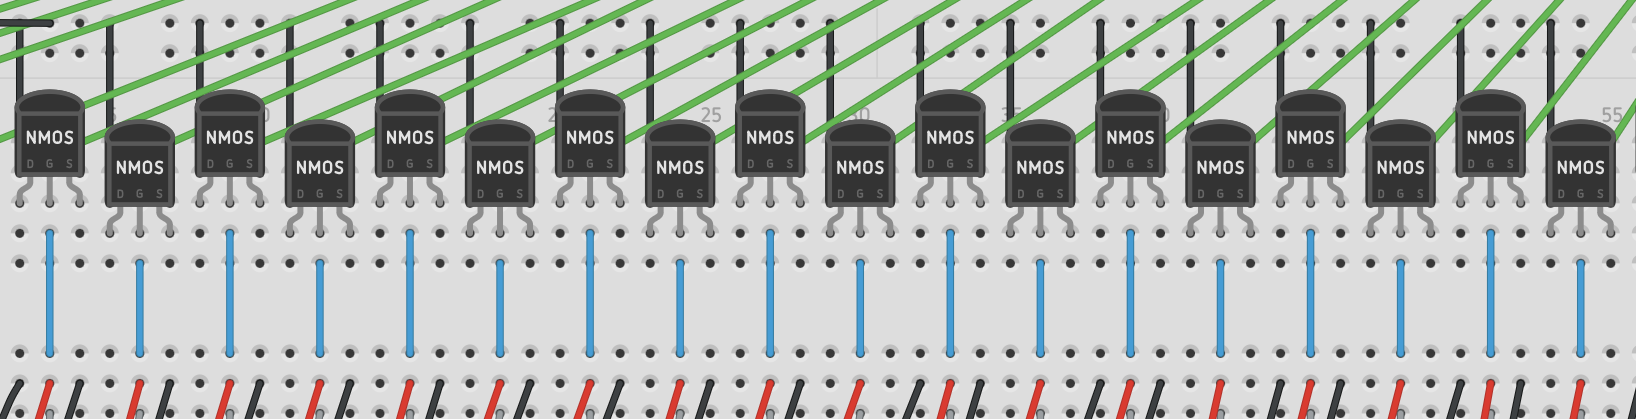
\includegraphics[width=0.9\textwidth]{img/MosSchaltung}
	\caption{Schaltung der Mosfets}
	\label{fig:SchaltungMosfet}
\end{figure}

\subsubsection{Hubmagnet}

Um den Stromkreis zu schließen wird der andere Kontakt des Hubmagnetes mit dem +24V verbunden.
Bei Hubmagneten ist es in der Regel egal, welcher Anschluss an Plus und welcher an Minus angeschlossen wird
(siehe Kapitel \ref{subsec:aktuator}).

\subsubsection{Testen}

Um die Fehlersuche zu erleichtern, werden LEDs in den Schaltplan mit eingebaut.
Diese werden jeweils mit einem entsprechenden $1k\Omega$ Widerstand parallel zu den Motoren angeschlossen.
So kann anhand der Helligkeit der LED die Intensität abgelesen werden, mit der eine Taste gespielt wird.
\newline

Für insgesamt 4 Hubmagnete (Wobei in dem Schema Motoren gewählt wurden, da das Programm keine Hubmagnete als Komponenten
zur Verfügung stellt) und 2 Schieberegister sieht die Darstellung des Schaltplans Schematisch wie folgt aus:

\begin{figure}[htbp]
	\centering
	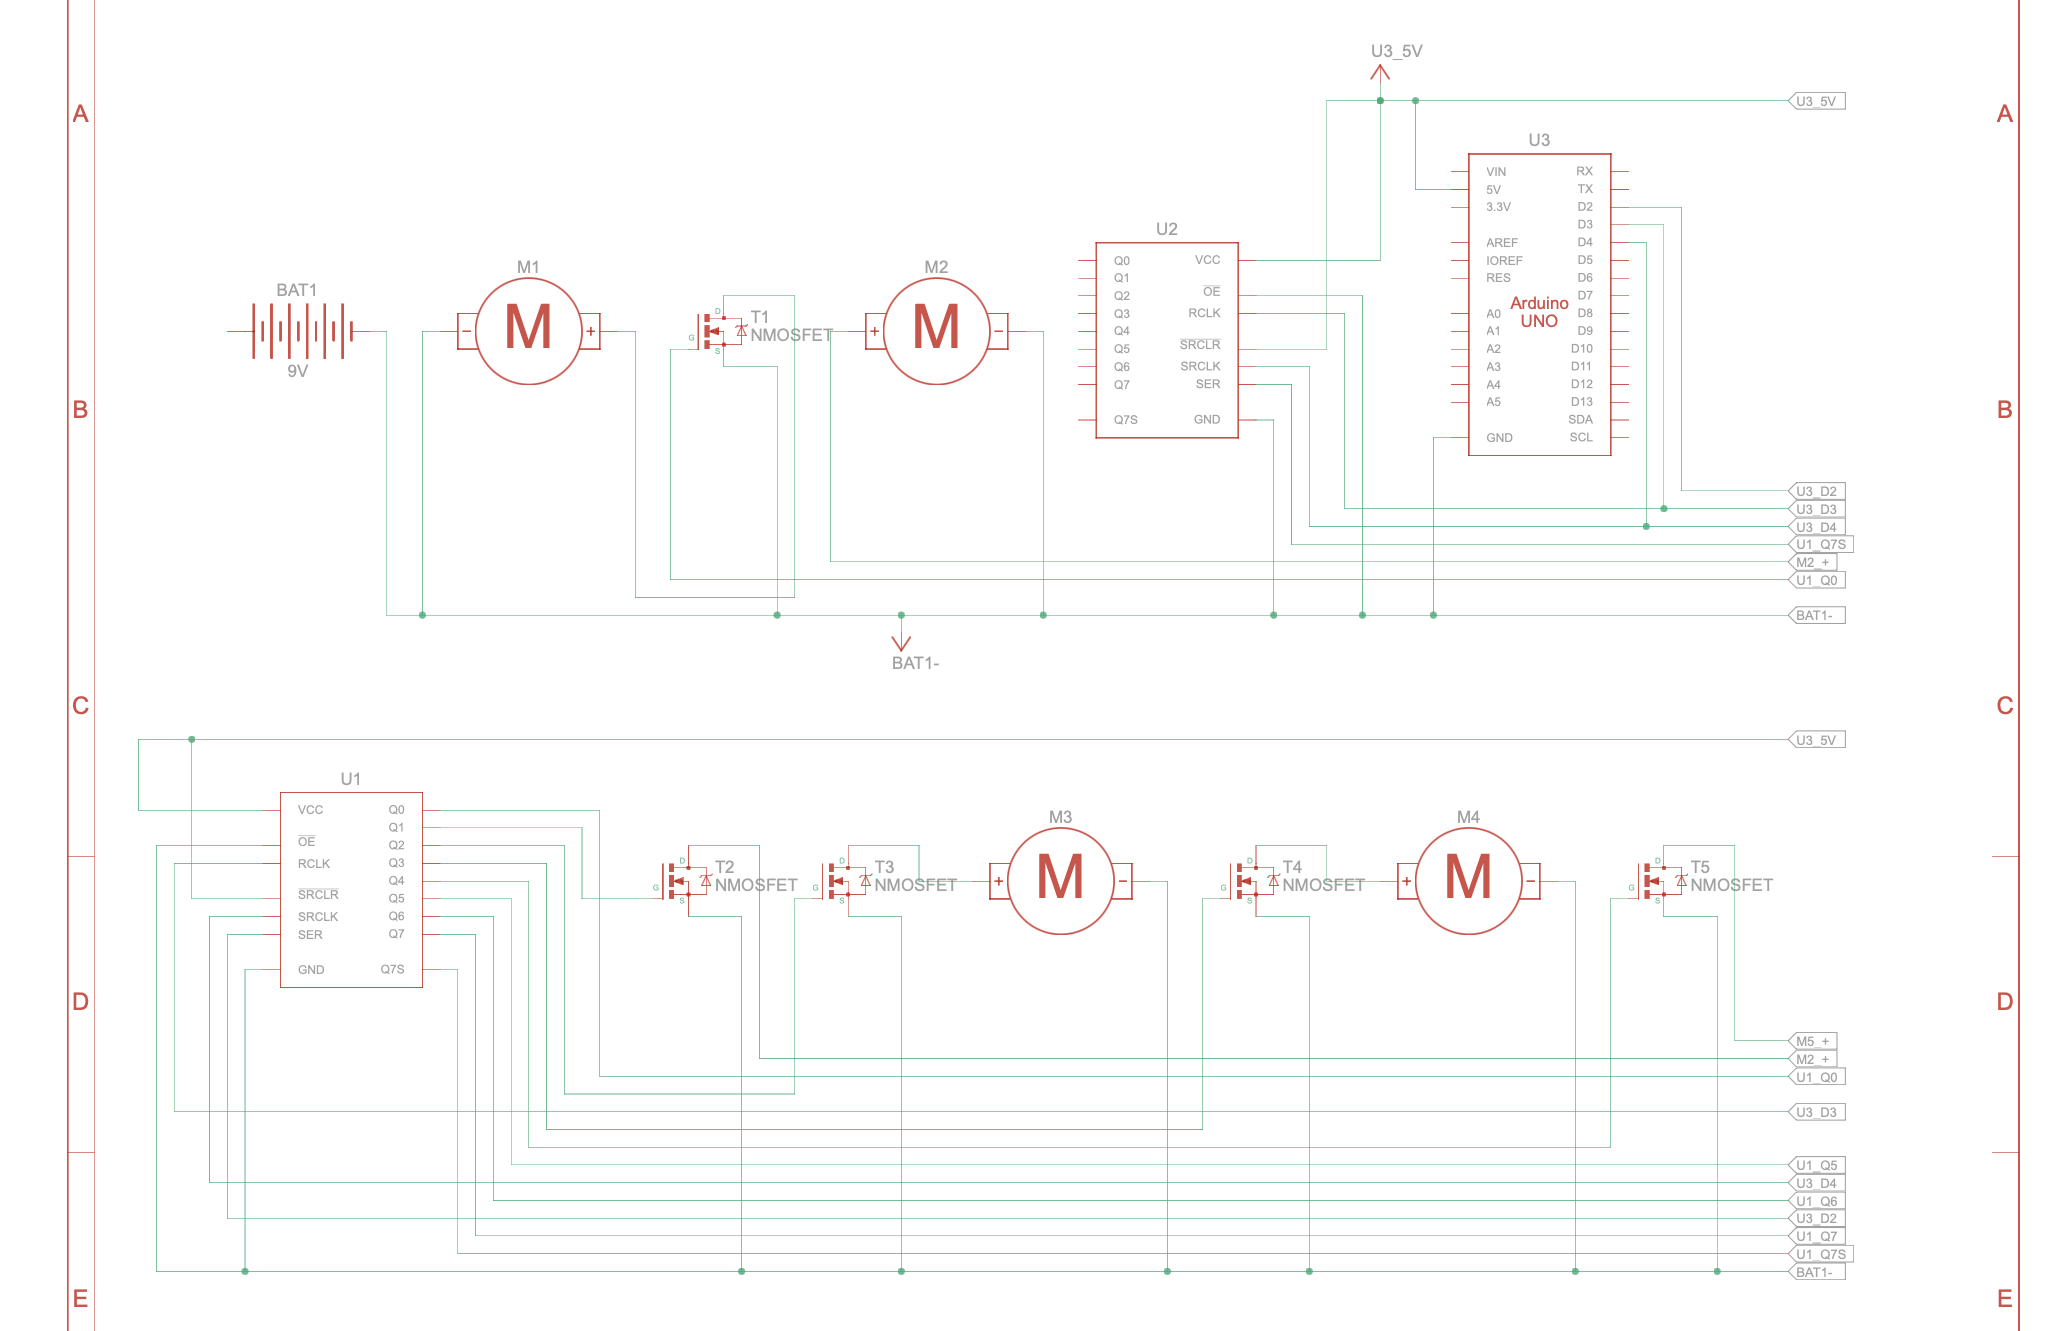
\includegraphics[width=0.9\textwidth]{img/SchematischeSchaltungExp}
	\caption{Beispielhaftes Schema des Schaltplans}
	\label{img:SchaltungExpSchema}
\end{figure}


